\documentclass[12pt]{article}

\usepackage[english]{babel}
\usepackage[utf8x]{inputenc}
\usepackage{amsmath}
\usepackage{enumitem}
\usepackage{graphicx}
\usepackage{ulem}
\usepackage{caption}
\usepackage{placeins}
\usepackage[usenames,dvipsnames]{color}
\usepackage[colorinlistoftodos]{todonotes}
\usepackage{listings}
\usepackage{fixltx2e}
\usepackage{scrpage2}
\usepackage{lastpage}
\usepackage{glossaries}

\clearscrheadfoot
\pagestyle{scrheadings}
\usepackage[
top    = 2.75cm,
bottom = 2.00cm,
left   = 2.50cm,
right  = 2.00cm]{geometry}
\setcounter{secnumdepth}{4}

\begin{document}
\begin{titlepage}
\begin{center}
% Oberer Teil der Titelseite:

\includegraphics[width=0.9\textwidth]{images/vwlogo}\\[1cm]    


% Title
\rule{1.0\textwidth}{1mm}
{ \huge \bfseries \\[0.4cm]  \huge ERP-Evaluation \\[0.4cm] }
\LARGE TGM - HTBLuVA Wien XX \\ IT Department  \\[0.4cm]

\rule{1.0\textwidth}{1mm}




% Author and supervisor
\noindent 
\vspace{3cm}

\begin{center}
\large
Authors: \\ 
Bergler \textsc{Adrian} \&
Haidn \textsc{Martin} \&
Siegel \textsc{Hannah} \&
Soyka \textsc{Wolfram}
\end{center}

\vfill

% Bottom of the page
{\large \today}

\end{center}
\end{titlepage}

\tableofcontents


%HEADER AND FOOTER
\pagenumbering{arabic}
\ohead{\headmark}
\automark{section}
\ifoot{© Bergler, Haidn, Siegel, Soyka}
\ofoot{\pagemark ~of \pageref{LastPage}}

\newpage

\section{Auswahl des Unternehmens}

\section{Volkswagen AG}
http://www.economist.com/node/21558269
\subsection{Das Unternehmen}
Die Volkswagen AG, ist Europas größter Automobilhersteller. Zum Volkswagen-Konzern gehören die Marken Audi, Bentley, Bugatti, Lamborghini, Seat, Skoda, Volkswagen und Volkswagen Nutzfahrzeuge. Allein in Deutschland gibt es neun Volkswagenwerke.

\subsubsection{Historie}
Der Volkswagen - die Idee, die relativ neue Erfindung der Automobilität in Form eines Wagens der für den kleinen Mann bezahlbar sei an selbigen zu bringen - kam erstmals im um 1904 herum auf. Allerdings vergingen 33 Jahre bis im Mai 1937 dazu dann die „Gesellschaft zur Vorbereitung des Deutschen Volkswagen mbH“ gegründet, welche im Jahr darauf in „Volkswagenwerk GmbH“ umbenannt wurde.\cite{vwchronik} \\
In Wolfsburg wurde das VW-Werk errichtet, wo der sogenannte KdF-Wagen (Kraft durch Freude), der größtenteils vom Konstrukteur Ferdinand Porsche konzipiert war, hergestellt wurde. Von Anfang an war den Herstellern allerdings aus vorhergehenden Versuchen diverser Automobilherstellern klar, dass der von Hitler geforderte Preis von höchstens 1000 Reichsmark nicht eingehalten werden konnte. \cite{geschdautos}\\
Während des 2.Weltkrieges wurde aufgrund von neuen Prioritäten und Ressourcenmangel die Herstellung von Autos im VW Werk größtenteils gestoppt und stattdessen auf Rüstungsgüter umgestellt, unter anderem auch auf Produktion der Vergeltungswaffe V1.\cite{autowp} Während dem 2. Weltkrieg wurde außerdem das KZ Arbeitsdorf nahe dem VW Werk erbaut, um das Werk mit Arbeitskräften zu versorgen.\cite{terror}  
\\
Nach dem Krieg werden im VW Werk (wieder) Autos gebaut. Innerhalb von 10 Jahren schafft es VW nicht nur das Werk von Kriegsschäden zu reparieren, sondern auch eine Million Käfer zu produzieren. \cite{ahwest}\\
Am 22. August 1960 wurde aus der "Volkswagen GmbH" eine Aktiengesellschaft, neun Jahre Später übernahm VW die Auto Union GmbH, der die Marke Audi gehörte. Seit diesem Zeitpunkt hat der Volkswagen Konzern mehr als eine Marke Autos im Angebot, was sich im laufe der nächsten Jahre auf stolze 12 Marken erhöhte (Stand Dez. 2013). \cite{vwag}
Die nächsten zwei Jahrzehnte war es vergleichsweise Ruhig um  Volkswagen, der in dieser Zeit allerdings keineswegs untätig war sondern u.a. das Erfolgsauto Golf und Passat hervorbrach und weitere Marken akquirierte, bis der Konzern im Geschäftsjahr 2003 einen Gewinneinbruch von 50 \% erlitt. Gründe hierfür waren laut VW notwendige Restrukturierungen in Brasilien, eine Rekordzahl an neuen Modellen und eine schlechte Situation am Weltmarkt. \cite{sud} \\
Zwei Jahre später hatte sich der Konzern zwar halbwegs von den Gewinneinbußen erholt, allerdings schrieb er wieder schlechte Schlagzeilen mit einem Korruptionsskandal und Umfassenden Streiks in einem Brasilianischen Werk. \cite{autowp}\\
2014 schaffte es VW mit 10,14 Millionen verkauften Fahrzeugen einmal mehr nur auf den zweiten Platz der größten Automobilhersteller der Welt, knapp hinter Toyota mit 10,23 Millionen verkauften Fahrzeugen. Das Toyota 2015 allerdings mit Einbußen im Heimatland Japan rechnet könnte es VW 2015 schaffen erstmals der größte Autohersteller der Welt zu werden.

\subsection{Finanzen}
%  3 u 4
\textbf{Umsatz}\\
Im Jahr 2013 lag der Umsatzerlös bei 65.587 Millionen Euro. Im Jahr zuvor jedoch betrug dieser 68.361 Millionen Euro. Ein Rückgang von 226 Millionen Euro ist dadurch entstanden. Gleichzeitig ist auch ein Gewinnrückgang von mehr als 3 Milliarden Euro festzuhalten. Gründe dafür lassen sich wie folgt finden:
\\
"Die in Vorjahren erworbenen 73,7\% der Anteile am Grundkapital der MAN SE, München, (9,1 Mrd.\euro) wurden von
der Volkswagen AG im Geschäftsjahr in die Truck \& Bus GmbH, eine 100-prozentige Tochtergesellschaft eingebracht.
Zusätzlich hat die Volkswagen AG 3,3 Mrd.\euro in die Kapitalrücklage der Truck \& Bus GmbH eingezahlt. Von der Truck \&
Bus GmbH wurden 2013 insgesamt 1,0 Mrd. \euro Verluste aufgrund des Beherrschungs- und Gewinnabführungsvertrags
mit der MAN SE übernommen. ",\cite[Seite 3]{jbilanz2013vw}
\\\\
"Die Volkswagen AG hat von der Volkswagen Bank GmbH, Braunschweig, eine Beteiligung erworben und diese anschließend im Wege der Sacheinlage (1,7 Mrd.\euro) in die VW Finance Luxemburg S.A., Luxemburg, eingebracht.\\
Darüber hinaus wurden Kapitalzuführungen bei der AUDI AG, Ingolstadt, (1,9 Mrd.\euro) und kleinere Kapitalmaß-
nahmen bei verbundenen Unternehmen durchgeführt. Bei der der Global Automotive C.V. Amsterdam, Niederlande
wurde eine Sachkapitalherabsetzung. (1,1 Mrd.\euro) durchgeführt. Die Volkswagen AG hat im HI-TV Fonds (TreasuryFonds) 1,0 Mrd.€ angelegt. ",\cite[Seite 4]{jbilanz2013vw}
\\ \\ 
\textbf{Aktie} \\
"On 7 April 1961, the Volkswagen Share was traded for the first time on a regulated open market, thus writing a chapter of economic history.",\cite{vsc50y} \\
\\
Marktkap. total (Stamm + Vorzug): EUR 114,71 Mrd.
\begin{figure}[here!]
\centering
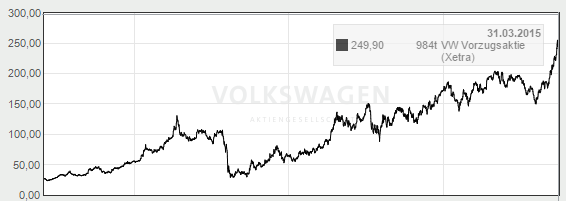
\includegraphics[width=0.7\textwidth]{images/finanzen2015}
\caption{Zehn Jahres Übersicht der VW-Vorzugsaktie \cite{aktienfotos}}
\label{fig:vwaktie1}
\end{figure}\FloatBarrier
\noindent
Wie in Abbildung \ref{fig:vwaktie1} zu sehen ist, ist die Volkswagen Vorzugsaktie in den letzten zehn Jahren stetig gestiegen. In 2008 wurde der Fall der Aktie durch die Finanzkrise bedingt.\\
Der Stand am Dienstag, dem 31. März 2015, der VW Vorzugsaktie (Xetra) war bei 249,90 \euro.
\begin{figure}[here!]
\centering
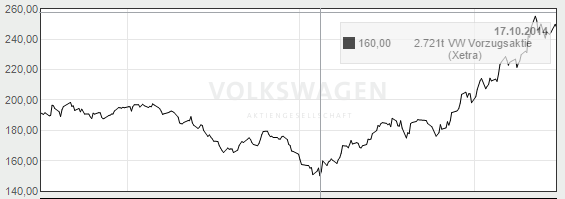
\includegraphics[width=0.7\textwidth]{images/finanzen20151}
\caption{Jahres Übersicht der VW-Aktie \cite{aktienfotos}}
\label{fig:vwaktie3}
\end{figure}\FloatBarrier
\noindent
Im letzten Jahr war das minimum im Oktober bei 160 \euro erreicht. Seit diesem Tag ist sie auch stetig bis auf kleine Ausnahmen gestiegen.
\begin{figure}[here!]
\centering
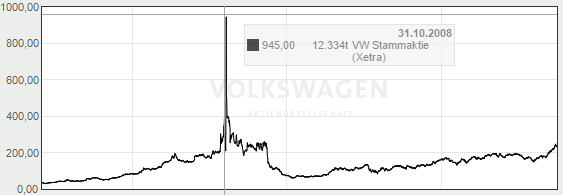
\includegraphics[width=0.7\textwidth]{images/finanzen2015S}
\caption{Zehn Jahres Übersicht der VW-Stammaktie \cite{aktienfotos}}
\label{fig:vwaktie2}
\end{figure}\FloatBarrier
\noindent
%TODO mama fragen
%(Reuters) - Volkswagen (VOWG.DE) briefly became the world's biggest company by market value on Tuesday, as short sellers caught betting on a price drop with borrowed stock scrambled to find shares after a buying spree by Porsche (PSHG_p.DE).Short sellers desperate to close their positions paid as much as 1,005 euros a share during the session following Sunday's news that there was less than 6 percent of VW voting stock still floating in the market.At that price Volkswagen's voting stock was worth 296 billion euros ($370 billion), or more than the $343 billion market capitalization of Exxon Mobil (XOM.N). VW shares later closed trading on Tuesday up 82 percent at 945 euros.
% % % \cite{2008wtf} % % %
\textbf{Aktinonärsstruktur}\\
Mit 31.12.2014 waren insgesammt 180.641.478 Vorzugsaktien und 295.089.818 Stammaktien ausstehend.\\
Im Juni 2014 hat die Volkswagen Aktiengesellschaft 10.471.204 neue Vorzugsaktien ausgegeben. Zusätzlich wurden im 1. Halbjahr 2014 22.103 Vorzugsaktien aus der Wandlung von Pflichtwandelanleihen geschaffen. Zum Stichtag 30. Juni 2014 setzte sich das gezeichnete Kapital der Volkswagen Aktiengesellschaft aus 295.089.818 Stammaktien und 180.641.478 Vorzugsaktien zusammen.
\cite{aktionaersstruktur} \\ \\
\textit{Stimmrechtsverteilung} \\
50,73\% Porsche Automobil Holding SE, Stuttgart\\
20,00\% Land Niedersachsen, Hannover\\
17,00\% Qatar Holding LLC\\
12,30\% Weitere
\\ \\
\textbf{Recovery}\\
"When Ferdinand Piëch arrived as Volkswagen's chief executive in 1993, things looked dire. The carmaker was overspending, overmanned and inefficient, and had lost its reputation for quality. How things have changed: last year the VW group's profits more than doubled, to a record €18.9 billion (\$23.8 billion). As other European volume carmakers seek to close factories and cut jobs, VW is seizing market share in Europe, booming in China and staging a comeback in America. It plans to spend €76 billion on new models and new factories by 2016. Its global workforce is more than half a million, and growing."\cite{ec2}
\\ \\
\textbf{Sales in America} \\
"The firm reported some of its best sales figures since the era of the original Beetle—and said it wanted to sell at least 800,000 vehicles per year in America by 2018.\\
Then, rather suddenly, things went south. Although Volkswagen of America is still well ahead of where it was before the Great Recession, it has suffered two consecutive years of declining sales. And in the first five months of 2014, as rivals such as GM posted some of their best numbers in a decade, the VW brand’s sales dropped by another 15\%. With sales in America barely above 400,000 in 2013, down 7\% from the previous year, doubts have been growing as to whether VW will be able to reach its target of 800,000 by 2018." \cite{ec1}

\newpage
\begin{table}
\begin{tabular}{|p{0.4\textwidth}|p{0.4\textwidth}|}
\hline
\textbf{Geschäftsjahr}  & \\  \hline
Geschäftsjahresende &   31. Dez \\  
Letztes Quartal (mrq) &   31.12.2014 \\  
Geschäftsjahresende &   31. Dez \\  \hline
\textbf{Rentabilität}  & \\  \hline
 Gewinnspanne (ttm)&   5,89\% \\  
 Operative Marge (ttm)&	5,89\%    \\ \hline
 \textbf{Managementeffektivität}  & \\  \hline
Kapitalrentabilität (ttm) & 2,21\%  \\  
Eigenkapitalrendite (ttm) &   12,28\%  \\  \hline
 \textbf{GuV}  & \\  \hline

 Umsatz (ttm)&   202,46Mrd. \\  
 Umsatz pro Aktie (ttm)&  408,12  \\  
 
Vierteljährliches Umsatzwachstum (yoy)&   6,60\% \\  
 Bruttoergebnis vom Umsatz (ttm)&34,39Mrd.    \\  
EBITDA (ttm)6 &  20,50Mrd.  \\  
 Auf Stammaktien entfallender Jahresüberschuss (ttm) &  10,98Mrd.  \\  \hline
  \textbf{Bilanz}  & \\  \hline


Cash (gesamt) (mrq): &  	28,30Mrd.  \\  

Gesamt-Cash pro Aktie (mrq): & 59,50   \\  
Schulden (gesamt) (mrq): &   108,65Mrd. \\  
 Schulden/Equity (gesamt) (mrq):&  	120,47  \\  \hline
   \textbf{Cash Flow-Aufstellung}  & \\  \hline

Cash Flow aus betrieblichen Tätigkeiten (ttm) &  10,78Mrd.  \\  
Levered Free Cash Flow (ttm) &  8,45Mrd.  \\  \hline

\end{tabular}
\end{table}
\cite{yahoofinanzenvw}

\subsection{Produktspektrum}
Im Mittelpunkt der Produktion steht das Automobil und wird von eine Anzahl an vielseitigen Dienstleistungen rund um das Thema Fahren verstärkt.
Das Produktspektrum der Volkswagen AG beinhaltet alle Kfz vom Stadtfahrzeug, über Motorad, bis zum Großtransporter.
So unterteilt sich der Konzern in die Folgenden Marken und Tochtergesellschafen.
\begin{figure}[here!]
\centering
% 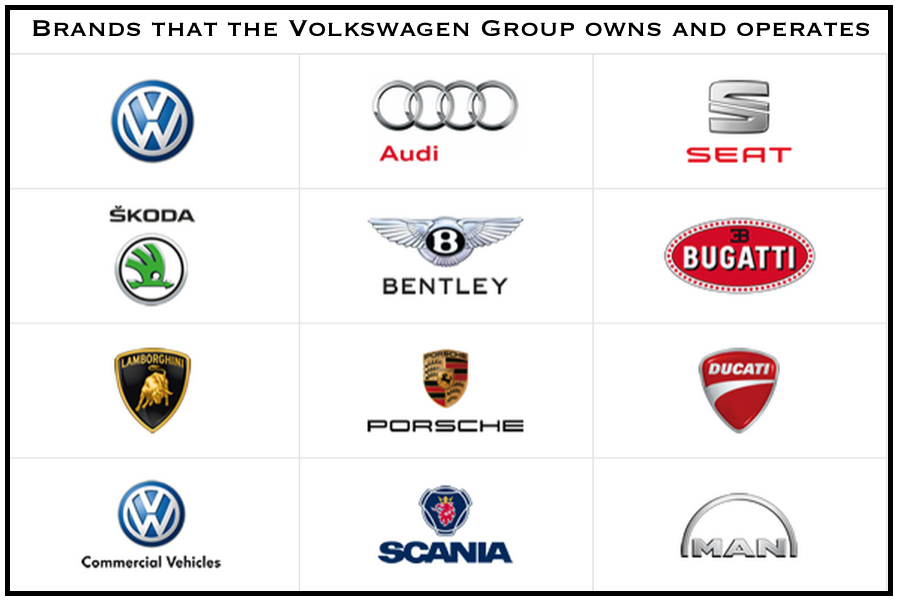
\includegraphics[width=0.7\textwidth]{images/Volkswagen-Group-Brands} %TODO
\caption{Marken und Tochtergesellschaften der Volkswagen AG. \cite{marken}}
\end{figure}\FloatBarrier
\noindent
\textbf{Volkswagen Group}\\
Das Segment der Volkswagen Group ist überwiegend auf den Endverbaucher Abgestimmt. Es beinhaltet den kleinen Stadtflitzer bis zum SUV. Die klingensten Modelle darunter sind unter anderem Käfer, Polo, Golf, Passat und Sharan.
Auch im elektrifizierten Modellbereich ist die Marke mit der e-up! und e-golf Serie vertreten.\\
\\
\textbf{Audi}\\
Audi produziert seither in den gängigen Klassen A, S, T, Q und weitere Kleinserien in der typischen Buchstabenbenennung. Seit mittlerweile 60 Jahren der Produktion sind die Klassen in ihrer achten Generation angelangt und bietet seinen Fahrern eine weitgestreutet Modellpallette von Kleinwagen, über Sportwagen und SUV, bis zur Oberkalsse.\\
\\
\textbf{Skoda}\\
Die Modelle der Marke Skoda sind eher in der Mittelklasse orientiert, bieten dem Fahrer allerdings zu günstigeren Preisen als manche andere Konzerntöchter, eine Vielzahl von aktuellen Features und neuen technologien zum Fahrkomfort und Sicherheit.
Die gängisten Modelle sind Fabia, Rapid und Octavia.

\newpage
\textbf{Seat}\\
Der Spanische Marke Seat ist im Kleinwagen und Mittelklasseberreich zu Hause. Der überwiegende Teil der produzierten Serien sind Lizenzbauten der Marke Fiat und den Volkswagen eigenen Marken VW, Audi und Skoda.
Die gängigsten Serien der Marke sind unter anderen Ibiza und Leon.\\
\\ 
\textbf{Porsche}\\
Die Luksusmarke Porsche entwickelt ausschließlich Sportwagen, Oberklassenmodelle und SUV's.
Die gängisten Serien des Herstellers sind Cayenne, Boxter und 911, von denen Carriera die größte unterserie besitzt.\\
\\
\textbf{Lamborghini}\\
Der Luxushersteller produziert hauptsächlich Sportwagen und Coupes in Serie. Neben den Serienmodellen wurden auch eine
Vielzahl von Einzelmodellen entworfen, die in Design und Ergonomität, dafür aber auch Preis glänzen.\\
\\
\textbf{Bentley}\\
Der Hoflieferat für die brittische Königsfamilie, der ursprünglich lediglich als Marke der Firma Rolls-Royce bekannt war, ist seit  ist ebenfalls für seine Modelle in der Ober- und Sportklasse bekannt.

\textbf{Bukatti}\\
\textbf{Ducati}\\
\textbf{Scania}\\
\textbf{MAN}


\newpage
\subsection{Standorte und Unternehmensstruktur}
Der Konzern betreibt über 118 Fertigungsstätten in denen rund 600.000 Personen beschäftigt sind.
Der überwiegende Teil ist nach Afrika und Asien ausgelagert, der rest wird zum Teil in Amerika und Europa in den
folgenden Ländern Produziert. \cite{produktionsstandorte}
\begin{table}[h]
	\begin{tabular}{|l|l|l|l|l|}
		\hline
		Argentinien          & Bosnien und Herzegovina & Brasilien & China    & Deutschland          \\ \hline
		Indien               & Mexiko                  & Polen     & Portugal & Russische Föderation \\ \hline
		Slowakische Republik & Spanien                 & Südafrika & USA      &                      \\ \hline
	\end{tabular}
\end{table}
\\\\
"Die Volkswagen AG stellt die Muttergesellschaft des eigentlichen Volkswagen Konzerns da und entwickelt insbesondere Pkw und Nutzfahrzeuge für den Vertrieb, sowie Fahrzeuge und deren Komponenten für den Konzern.
"Der Vorstand der Volkswagen AG leitet das Unternehmen in eigener Verantwortung. Der Aufsichtsrat bestellt, überwacht und berät den Vorstand und ist in Entscheidungen, die von grundlegender Bedeutung für das Unternehmen sind, unmittelbar eingebunden." \cite{struktur}



\subsection{Logistik}
\newpage
\subsection{Unternehmensstruktur}
\subsubsection{Vorstand und Konzernleitung}
Die Volkswagen AG und der Volkswagen Konzern werden vom Vorstand der Volkswagen AG geleitet.
Weiters gibt es das Gremium Konzernleitung, das dafür Sorge trägt, dass die Konzerninteressen bei Entscheidungen der Marken und Gesellschaften des Konzerns beachtet werden. Es besteht aus den Mitgliedern des Vorstands und ausgewählten Top-Managern mit Konzernsteuerungsfunktionen.

\subsubsection{Vorsitzender des Vorstands der Volkswagen AG}
\textbf{Vorstands Vorsitzender}
\begin{figure}[here!]
	\centering
	\begin{minipage}[h]{0.20\textwidth}
		\centering
		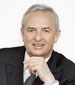
\includegraphics[width=1.0\textwidth]{images/MartinWinterkorn.jpg}
		\label{fig:vorstandvw0}
		\cite{mwpic}
	\end{minipage}
		\begin{minipage}[h]{0.10\textwidth}
		\hspace{1cm} 
	\end{minipage}
	\begin{minipage}[h]{0.65\textwidth}
		Prof. Dr. Dr. h. c. mult. Martin Winterkorn\\
		Mitglied des Vorstands der Volkswagen AG,\\
		Geschäftsbereich 'Konzern Forschung und Entwicklung',\\
		Vorsitzender des Aufsichtsrats der AUDI AG,\\
		Vorsitzender des Vorstands der Porsche Automobil Holding 
	\end{minipage}
\end{figure}\FloatBarrier\noindent

\textbf{Mitglieder des Vorstands}
\begin{figure}[here!]
	\centering
	\begin{minipage}[h]{0.65\textwidth}
		Dr. rer. pol. h. c. Francisco Javier Garcia Sanz\\
		Geschäftsbereich 'Beschaffung'
	\end{minipage}
		\begin{minipage}[h]{0.10\textwidth}
		\hspace{1cm}
		\cite{fspic}
	\end{minipage}
	\begin{minipage}[h]{0.20\textwidth}
		\centering
		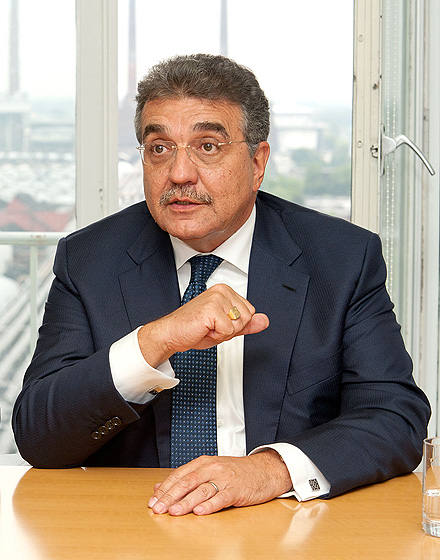
\includegraphics[width=1.0\textwidth]{images/FranciscoSanz.jpg}
		\label{fig:vorstandvw1}
	\end{minipage}
\end{figure}

\begin{figure}[here!]
	\centering
	\begin{minipage}[h]{0.20\textwidth}
		\centering
		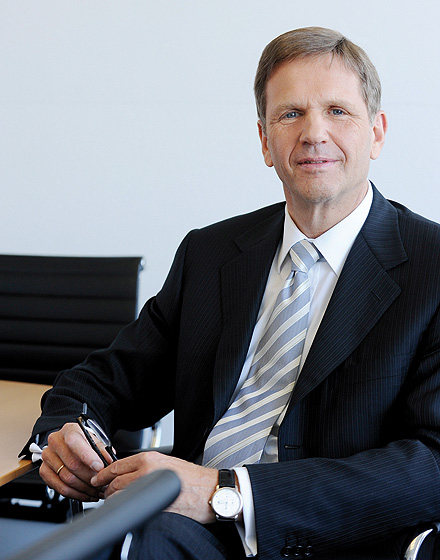
\includegraphics[width=1.0\textwidth]{images/JochemHeizmann.jpg}
		\label{fig:vorstandvw2}
		\cite{jhpic}
	\end{minipage}
	\begin{minipage}[h]{0.10\textwidth}
		\hspace{1cm} 
	\end{minipage}
	\begin{minipage}[h]{0.65\textwidth}
		Prof. Dr. rer. pol. Dr.-Ing. E. h. Jochem Heizmann\\
		Geschäftsbereich 'China'
	\end{minipage}
\end{figure}

\begin{figure}[here!]
	\centering
	\begin{minipage}[h]{0.65\textwidth}
		Christian Klingler\\
		Geschäftsbereich 'Vertrieb und Marketing'\\
		Mitglied des Markenvorstands Volkswagen\\
		Geschäftsbereiche 'Vertrieb, Marketing und After Sales'
	\end{minipage}
	\begin{minipage}[h]{0.10\textwidth}
		\hspace{1cm} 
	\end{minipage}
	\begin{minipage}[h]{0.20\textwidth}
		\centering
		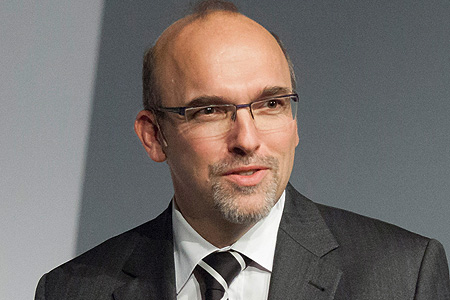
\includegraphics[width=1.0\textwidth]{images/ChristianKlingler.jpg}
		\label{fig:vorstandvw3}
		\cite{ckpic}
	\end{minipage}
\end{figure}

\begin{figure}[here!]
	\centering
	\begin{minipage}[h]{0.20\textwidth}
		\centering
		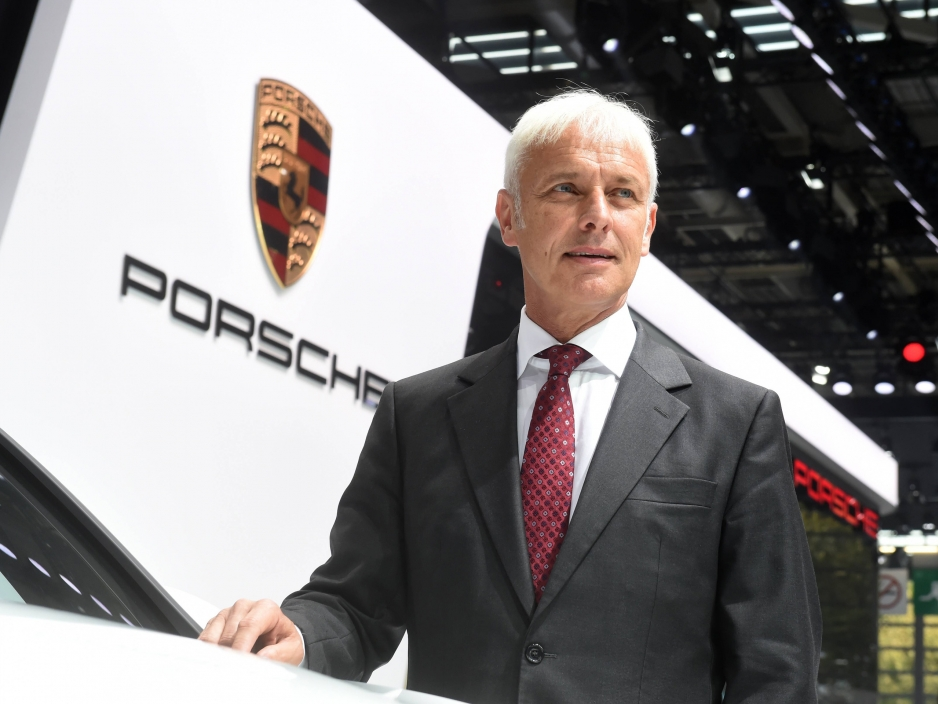
\includegraphics[width=1.0\textwidth]{images/MathiasMueller.jpg}
		\label{fig:vorstandvw4}
		\cite{mmpic}
	\end{minipage}
	\begin{minipage}[h]{0.10\textwidth}
		\hspace{1cm} 
	\end{minipage}
	\begin{minipage}[h]{0.65\textwidth}
		Matthias Müller\\
		'Vorstandsvorsitzender der Dr. Ing. h. c. F. Porsche AG'
	\end{minipage}
\end{figure}

\begin{figure}[here!]
	\centering
	\begin{minipage}[h]{0.65\textwidth}
		Prof. h. c. Dr. rer. pol. Horst Neumann\\
		Geschäftsbereich 'Personal und Organisation'
	\end{minipage}
	\begin{minipage}[h]{0.10\textwidth}
		\hspace{1cm} 
	\end{minipage}
	\begin{minipage}[h]{0.20\textwidth}
		\centering
		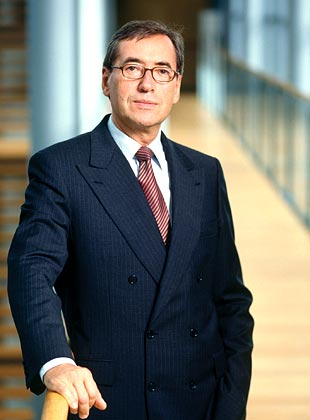
\includegraphics[width=1.0\textwidth]{images/HorstNeumann.jpg}
		\label{fig:vorstandvw5}
		\cite{hmpic}
	\end{minipage}
\end{figure}

\begin{figure}[here!]
	\centering
	\begin{minipage}[h]{0.20\textwidth}
		\centering
		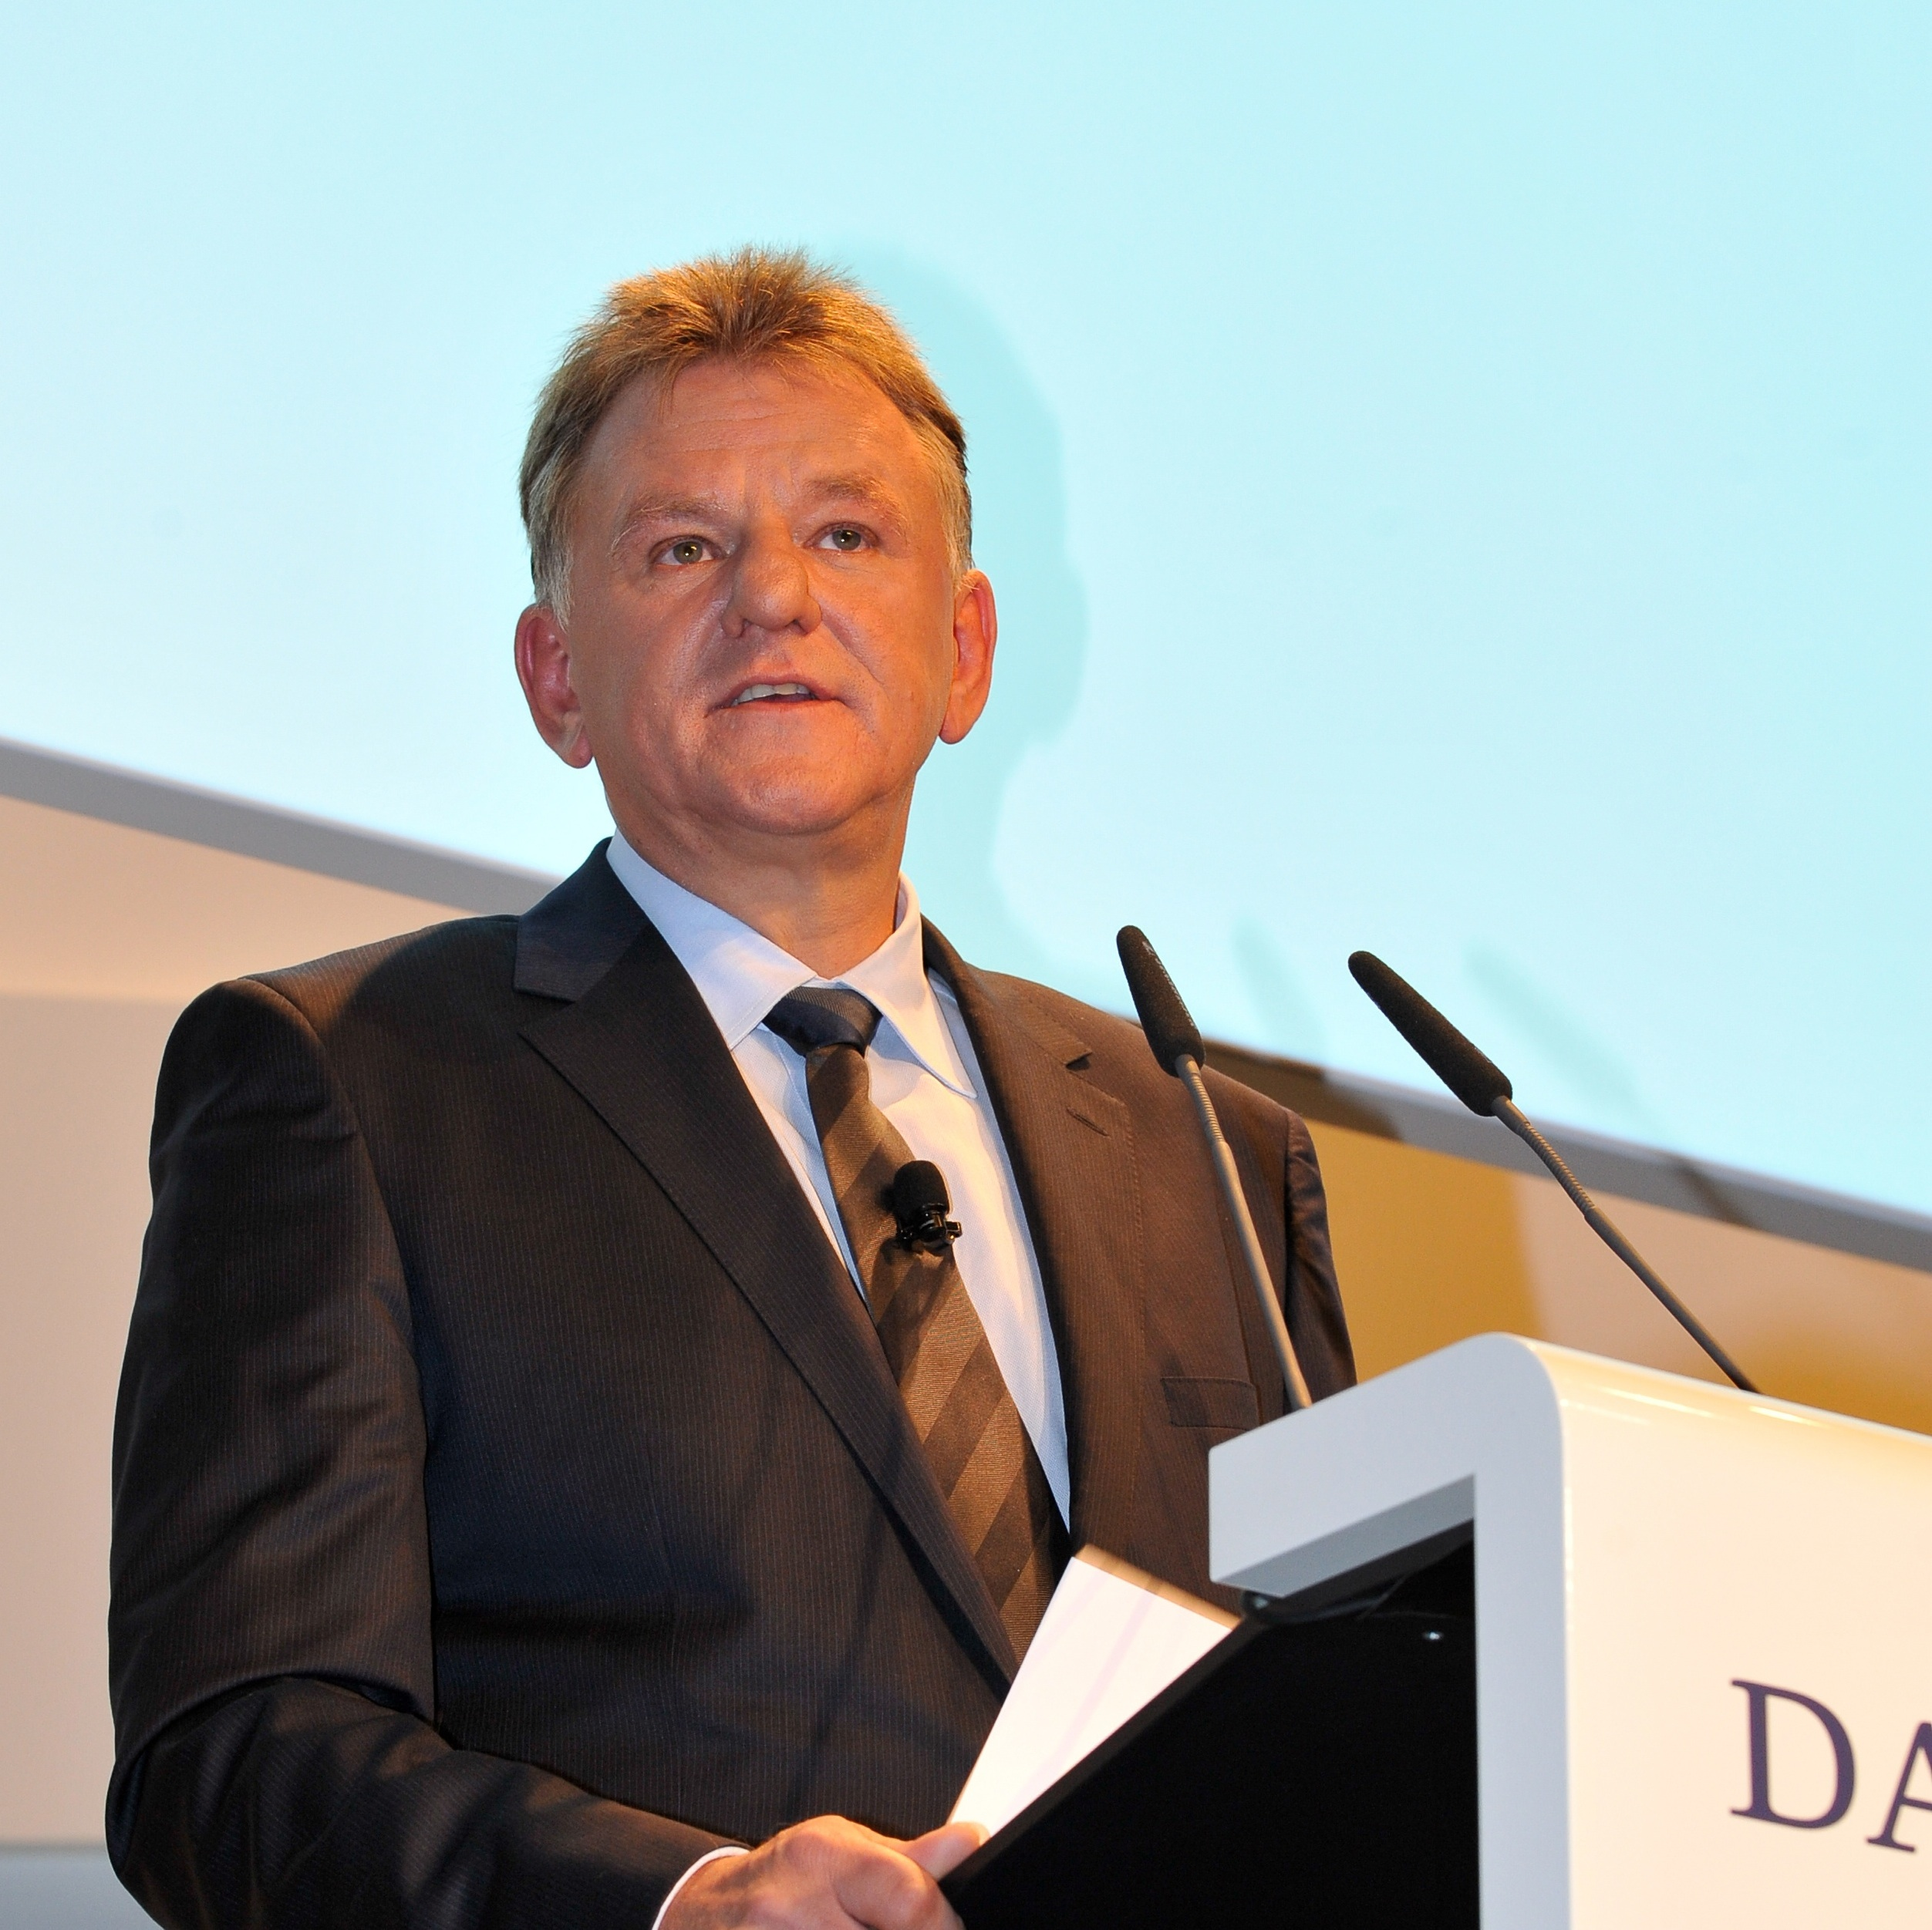
\includegraphics[width=1.0\textwidth]{images/AndreasRenschler.jpg}
		\label{fig:vorstandvw6}
		\cite{arpic}
	\end{minipage}
	\begin{minipage}[h]{0.10\textwidth}
		\hspace{1cm} 
	\end{minipage}
	\begin{minipage}[h]{0.65\textwidth}
		Andreas Renschler
		Geschäftsbereich 'Nutzfahrzeuge'
	\end{minipage}
\end{figure}

\begin{figure}[here!]
	\centering
	\begin{minipage}[h]{0.65\textwidth}
		Hans Dieter Pötsch\\
		Geschäftsbereich 'Finanzen und Controlling'\\
		Finanzvorstand der Porsche Automobil Holding SE
	\end{minipage}
	\begin{minipage}[h]{0.10\textwidth}
		\hspace{1cm} 
	\end{minipage}
	\begin{minipage}[h]{0.20\textwidth}
		\centering
		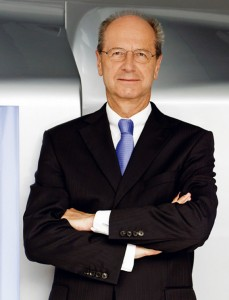
\includegraphics[width=1.0\textwidth]{images/HansPoetsch.jpg}
		\label{fig:vorstandvw7}
		\cite{dppic}
	\end{minipage}
\end{figure}

\begin{figure}[here!]
	\centering
	\begin{minipage}[h]{0.20\textwidth}
		\centering
		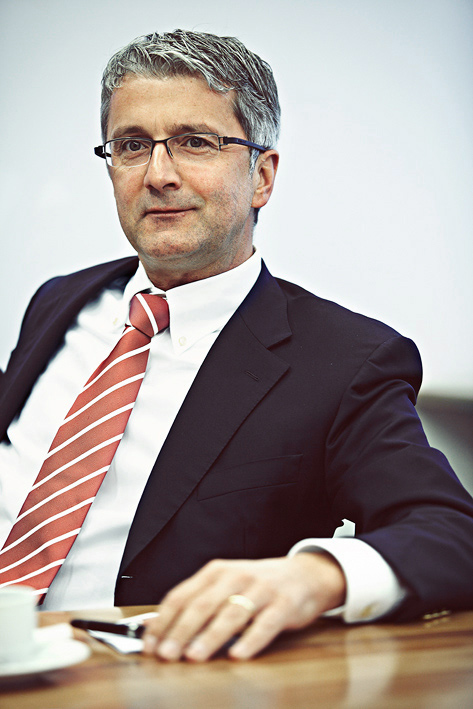
\includegraphics[width=1.0\textwidth]{images/RupertStadler.jpg}
		\label{fig:vorstandvw8}
		\cite{rspic}
	\end{minipage}
	\begin{minipage}[h]{0.10\textwidth}
		\hspace{1cm} 
	\end{minipage}
	\begin{minipage}[h]{0.65\textwidth}
		Prof. Rupert Stadler
		Vorstandsvorsitzender der Audi AG
	\end{minipage}
\end{figure}

\begin{figure}[here!]
	\centering
	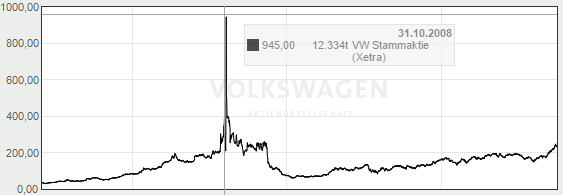
\includegraphics[width=0.7\textwidth]{images/finanzen2015S}
	\caption{Zehn Jahres Übersicht der VW-Stammaktie \cite{aktienfotos}}
	\label{fig:vwaktie2}
\end{figure}\FloatBarrier

\subsubsection{Marken und Hierarchie}
Jede Marke des Volkswagen Konzerns wird von einem Markenvorstand geleitet. Dabei sind die vom Vorstand der Volkswagen AG beziehungsweise von der Konzernleitung festgelegten Konzernziele und -vorgaben und die jeweiligen rechtlichen Rahmenbedingungen zu beachten. Angelegenheiten von konzernweiter Bedeutung werden der Konzernleitung vorgelegt.
Die einzelnen Gesellschaften des Volkswagen Konzerns werden jeweils unter Verantwortung einer eigenen Geschäftsleitung geführt. Dabei berücksichtigen die jeweiligen Geschäftsleitungen neben den Interessen der Gesellschaft auch Konzern- und Markeninteressen.\cite{structure1}
Die Hierarchie sieht dabei wie folgt aus:

\begin{table}[h]
	\begin{tabular}{|c|c|c|c|c|c|c|c|c|}
		\hline
		\multicolumn{9}{|c|}{Volkswagen AG}                                                                                                                                                     \\ \hline
		\multicolumn{3}{|c|}{Volkswagen} & \multicolumn{2}{c|}{Audi} & \multicolumn{2}{c|}{\begin{tabular}[c]{@{}c@{}}Volkswagen\\ Nutzfahrzeuge\end{tabular}} & \multicolumn{2}{c|}{Weitere} \\ \hline
		Skoda    & Bugatti   & Bentley   & Seat     & Lamborghini    & Scania                                       & MAN                                      & Suzuki       & Porsche       \\ \hline
	\end{tabular}
\end{table}

Die Volkswagen AG ist grundsätzlich schon immer durch die starke Eigenständigkeit der verschiedenen Marken geprägt. Die Marken sind beispielsweise für Produktdesign, Vertrieb, Marketing und vieles mehr weitgehend eigenständig. Sogar die Produktionsstandorte und Werke sind meistens einer einzelnen Marke zugeteilt und werden von dieser organisiert.
\cite{domavw}

\subsubsection{Logistik}

\subsection{Markt}
%Marktumfeld, -situation, -wert, Trends
Die Volkswagen Group, also alle Untermarken von VW gemeinsam produziert global am meisten PKWs, jedoch führt Toyota sowie General Motors noch vor Volkswagen den globalen, totalen Verkauf. 
In 2013 wurden von Volkswagen etwa 9.3 Millionen Autos produziert. \\
Toyota kommt aus Japan und dominiert sowohl den Japanischen als auch den amerikanischen Markt. GM kommt aus Amerika und produziert eher Pick Ups daher dominieren sie hier den Amerikanischen Markt.
\\\\
\textbf{Weltweit}\\
Wie in Abbildung \ref{fig:marktwelt} ersichtlich ist, führt Volkswagen den Marktanteil bei PKWs Weltweit an. 
\begin{figure}[here!]
\centering
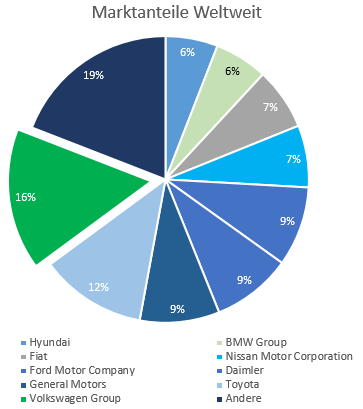
\includegraphics[width=0.7\textwidth]{images/maww}
\caption{Der Marktanteil Weltweit}
\label{fig:marktwelt}
\end{figure}\FloatBarrier
\noindent
\textbf{Europa}\\
Wie in Abbildung \ref{fig:markteuropa} ersichtlich ist, führt Volkswagen den Marktanteil in Europa bei weitem an. Diese Tendenz ist steigend.
\begin{figure}[here!]
\centering
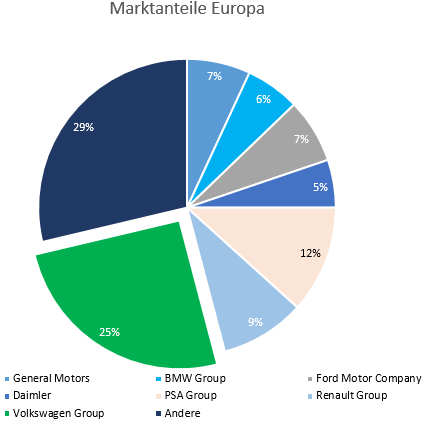
\includegraphics[width=0.7\textwidth]{images/maie}
\caption{Der Marktanteil in Europa}
\label{fig:markteuropa}
\end{figure}\FloatBarrier
\noindent
\textbf{Asia}\\
"Seit Beginn seiner Reform- und Öffnungspolitik vor über 30 Jahren ist China zu einem der wichtigsten Automobilmärkte der Welt aufgestiegen und bildet inzwischen den größten Absatzmarkt des Volkswagen Konzerns. Mit einem Anteil von 20,8 \% am Pkw-Markt und 3,27 Millionen verkauften Fahrzeugen im Geschäftsjahr 2013 ist der Volkswagen Konzern Marktführer in China."\cite{vwwebsitechina}\\
Durch das dort Ansässigle Unternehmen  Shanghai-Volkswagen Automotive Company (SVW) sowie des Unternehmens FAW-Volkswagen Automotive Company Ltd. (FAW-VW) konnten auch viele Produktionsstandorte in China verwendet werden.
Asien, insbesondere China zeichnet sich durch eine stetig steigende Nachfrage aus. So wurden inzwischen etwa 17 Gesellschaften (Komponenten-, Finanz- und Vertriebsgesellschaften) in Asien gegründet. \\
Ende der 90er Jahre wurde verstärkt mit der Diversifikation der Produktpalette begonnen. Das  Produktportfolio in Asien umfasst heute alle Segmente vom Kleinwagen bis zum Luxussportwagen.
\\
Mit seinem umfangreichen Produktportfolio, neuesten Technologien sowie den Planungen zu Hybrid- und Elektrofahrzeugen ist der Volkswagen Konzern bestens gerüstet, um zukünftigen Herausforderungen – zum Beispiel anspruchsvollen Emissionsgrenzen oder Zulassungsbeschränkungen in Megacitys – zu begegnen und auch langfristig eine Schlüsselrolle auf dem Automobilmarkt in Asien innezuhaben. \\ \\
\textbf{Japan} \\
Volkswagen konnte in Japan kaum Fuss fassen, unter anderem auch da Japan einige eigene Marken hervorgebracht hat.  Die Volkswagen Group kommt in Japan nur unter der Kategorie 'Andere' vor. Volkswagen selbst sieht jedoch das japanische Marksegment als nicht erstrebenswert zu erklimmen, da es sehr schwierig ist die lokalen Anbieter dort zu vertreiben.
\\\\
\textbf{Nordamerika}\\
Volkswagen konnte sich in Amerika noch nicht durchsetzten. Derzeit hat Volkswagen nur XXX \% des Marktanteiles (Verglichen mit 25\% in Europa) inne, wie man in Abbildung \ref{fig:marktnordamerika} sehen kann. Dies ist ein Ziel der kommenden paar Jahre. Die Autos haben zwar als Deutsche Qualitätsware einen guten Ruf, jedoch fehlt in Amerika auch die nötige Infrastruktur, also Händler und Werkstätten. \\ Desweiteren werden in Amerika mehr SUVs und Pick-Ups gekauft, ein Segment in welchem Volkswagen nicht unbedingt stark vertreten ist.
\begin{figure}[here!]
\centering
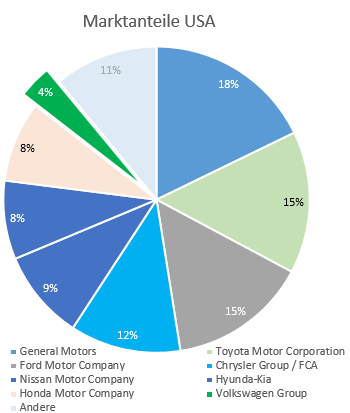
\includegraphics[width=0.7\textwidth]{images/maam}
\caption{Der Markt in den USA als Beispiel für Nordamerika}
\label{fig:marktnordamerika}
\end{figure}\FloatBarrier
\noindent

\subsection{Ziele und Zukunftsaspekte}
Laut der Volkswagen Website steht bis 2018 die Positionierung des Konzerns als weltweit führend sowohl ökonomisch und ökologisch.\\
Zur Erreichung dieser Ziele wurden vier Subziele (\cite{vwwebsitestrat}) definiert:
\begin{enumerate}
\item Steigerung der Kundenzufriedenheit und Qualität. Erreichung einer höheren Kundenzufriedenheit für nachhaltigen Erfolg.
\item Der Absatz soll von 9.259 Mio Fahrzeuge auf mehr als 10 Mio. Fahrzeuge gesteigert werden.  Vorallem auf die expandierenden Märkte in Asien soll ein stärkeres Augenmerk gelegt werden.
\item Die Umsatzrendite vor Steuern soll nachhaltig mindestens 8\% betragen, damit die finanzielle Solidität und Handlungsfähigkeit des Konzerns auch in schwierigen Marktphasen sichergestellt ist. % TODO ?
\item Volkswagen will sich auch als Arbeitgeber besser profilieren, um so besser qualifizierte Mitarbeiter gewinnen zu können.  \\\\
Des weiteren sind folgende Ziele immer wieder herauszusehen: \\
\item Volkswagen will auf dem amerikanischen Markt stärker present sein. Um genau dies zu schaffen, muss Volkswagen den Giganten Toyota vertreiben. \cite{ec1}
\item Volkswagen will in wachsenden Märkten vorallem mit dem neuen e-Golf und dem e-Up! Position beziehen. Elektro Fahrzeuge wurden Anfang 2000 noch kategorisch von der Firmenspitze abgelehnt. \cite{ec3} Dort sollen auch mehr Produktionsstandorte mit lokalen Zulieferern erbaut werden. 
\item Es sollen Umweltverträglichere und vorallem Spritsparende Autos entwickelt und produziert werden, um so mit dem derzeitigem globalen Trend von Nachhaltigkeit mithalten zu können. Durch ein Baukastensystem sowie einen Leichtbau des Fahrzeuges sollen neue ökologische Maßstäbe gesetzt werden.
\item Natürlich soll die führende Position von Volkswagen in Europa beibehalten werden und finanzielle Rücklagen gebildet werden.
\end{enumerate}

\section{Auswahl eines ERP Systemes}
\subsection{Auswahlkriterien}
\begin{figure}[here!]
\centering
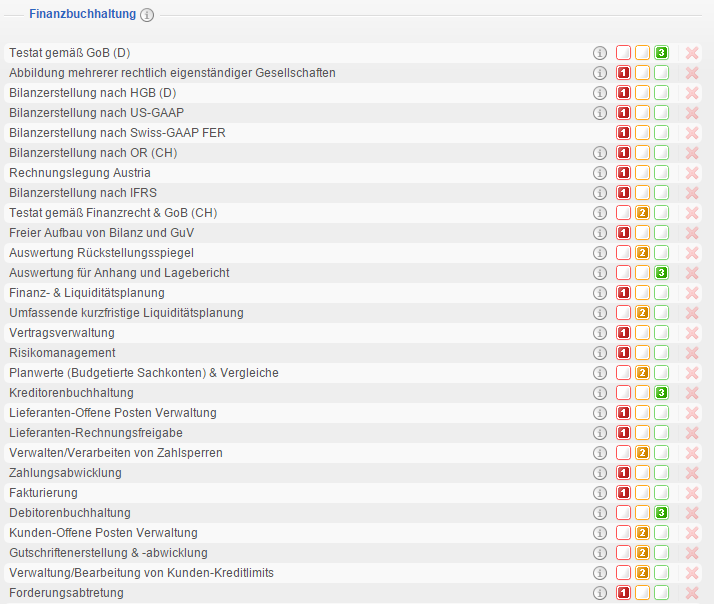
\includegraphics[width=0.7\textwidth]{images/tr1}
\end{figure}\FloatBarrier
\noindent
\begin{figure}[here!]
\centering
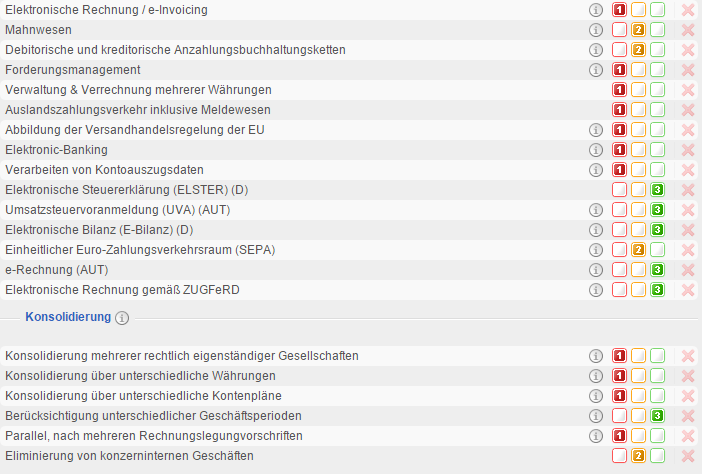
\includegraphics[width=0.7\textwidth]{images/tr2}
\end{figure}\FloatBarrier
\noindent
\begin{figure}[here!]
\centering
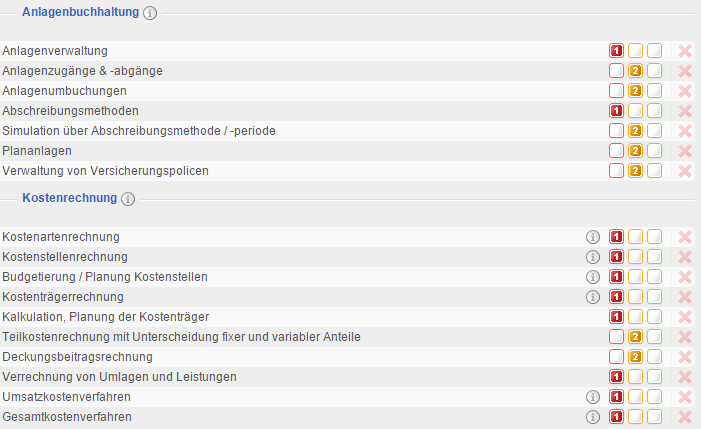
\includegraphics[width=0.7\textwidth]{images/tr3}
\end{figure}\FloatBarrier
\noindent
\begin{figure}[here!]
\centering
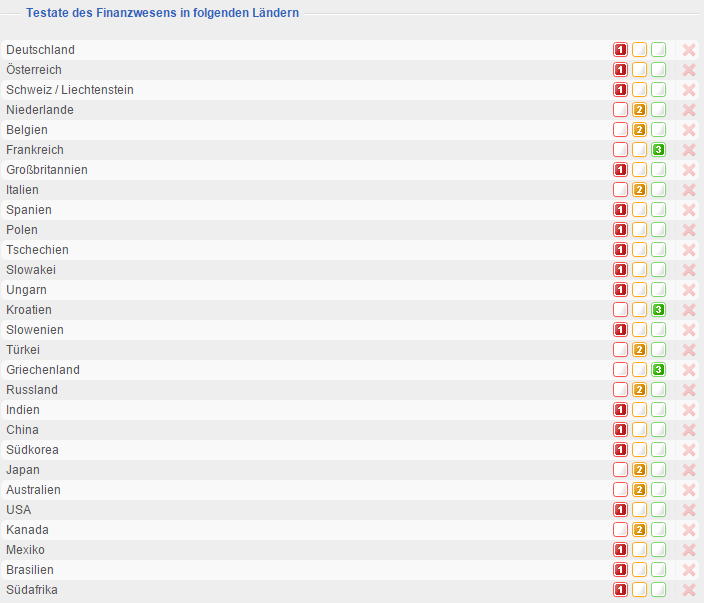
\includegraphics[width=0.7\textwidth]{images/tr4}
\end{figure}\FloatBarrier
\noindent
\begin{figure}[here!]
\centering
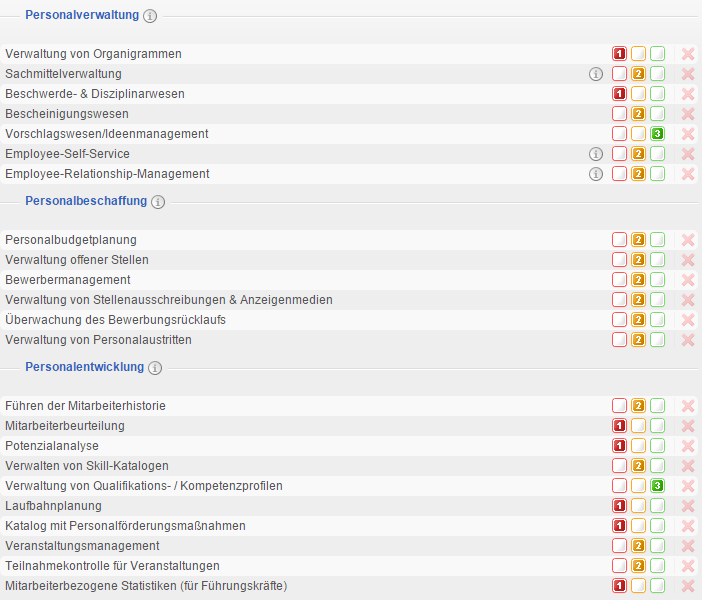
\includegraphics[width=0.7\textwidth]{images/tr5}
\end{figure}\FloatBarrier
\noindent
\begin{figure}[here!]
\centering
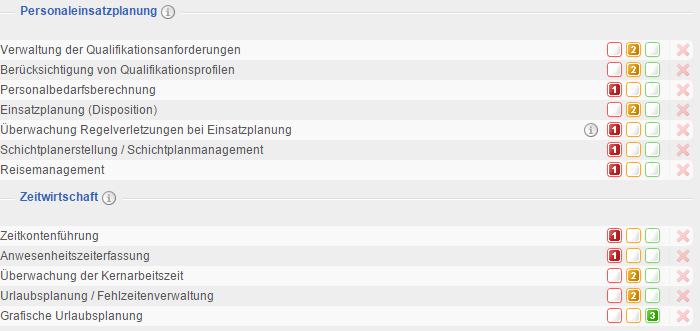
\includegraphics[width=0.7\textwidth]{images/tr6}
\end{figure}\FloatBarrier
\noindent
\begin{figure}[here!]
\centering
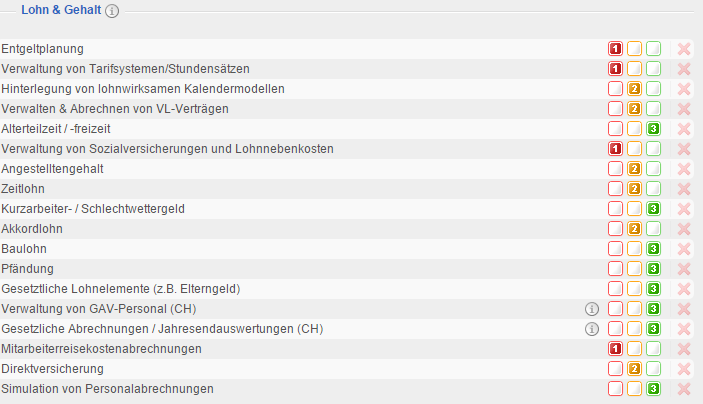
\includegraphics[width=0.7\textwidth]{images/tr7}
\end{figure}\FloatBarrier
\noindent
\begin{figure}[here!]
\centering
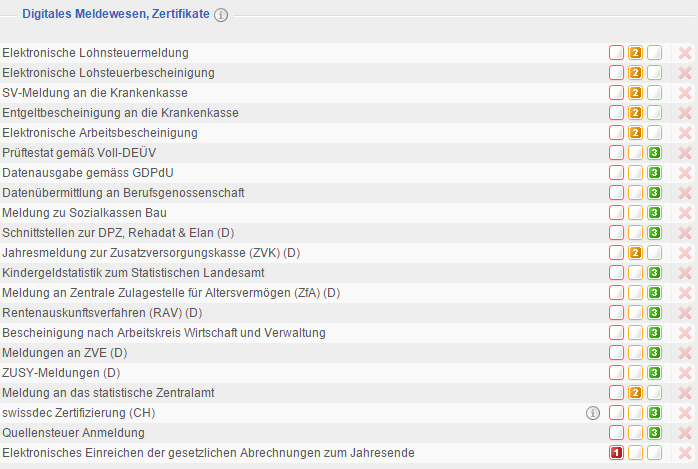
\includegraphics[width=0.7\textwidth]{images/tr8}
\end{figure}\FloatBarrier
\noindent
\begin{figure}[here!]
\centering
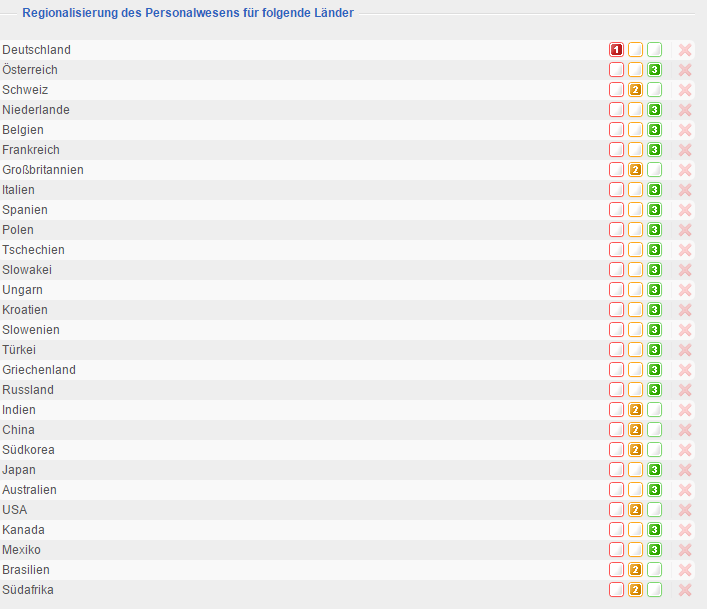
\includegraphics[width=0.7\textwidth]{images/tr9}
\end{figure}\FloatBarrier
\noindent
\begin{figure}[here!]
\centering
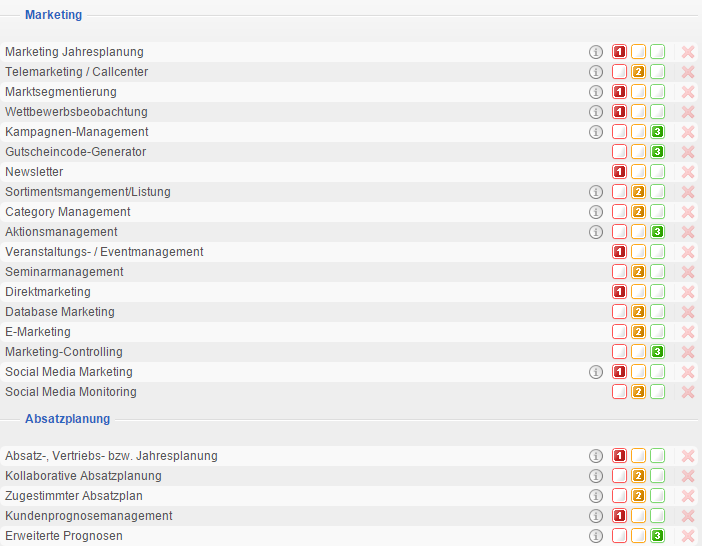
\includegraphics[width=0.7\textwidth]{images/tr10}
\end{figure}\FloatBarrier
\noindent
\begin{figure}[here!]
\centering
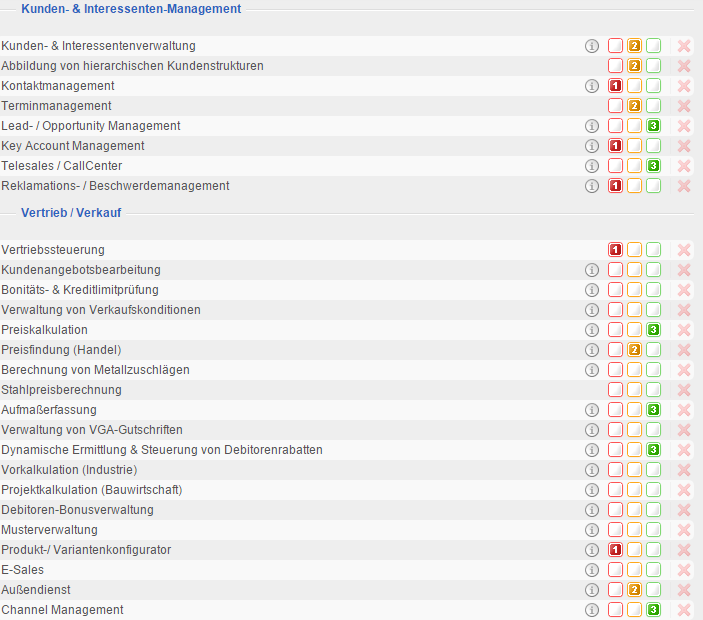
\includegraphics[width=0.7\textwidth]{images/tr11}
\end{figure}\FloatBarrier
\noindent
\begin{figure}[here!]
\centering
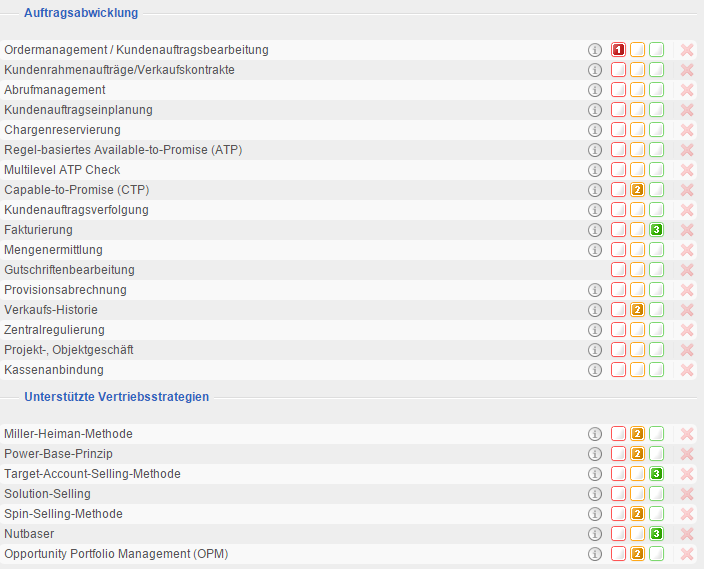
\includegraphics[width=0.7\textwidth]{images/tr12}
\end{figure}\FloatBarrier
\noindent
\begin{figure}[here!]
\centering
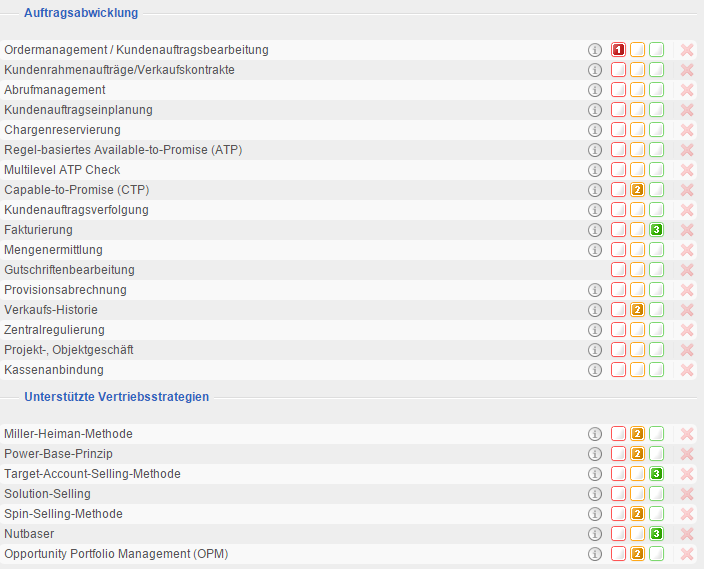
\includegraphics[width=0.7\textwidth]{images/tr13}
\end{figure}\FloatBarrier
\noindent
\begin{figure}[here!]
\centering
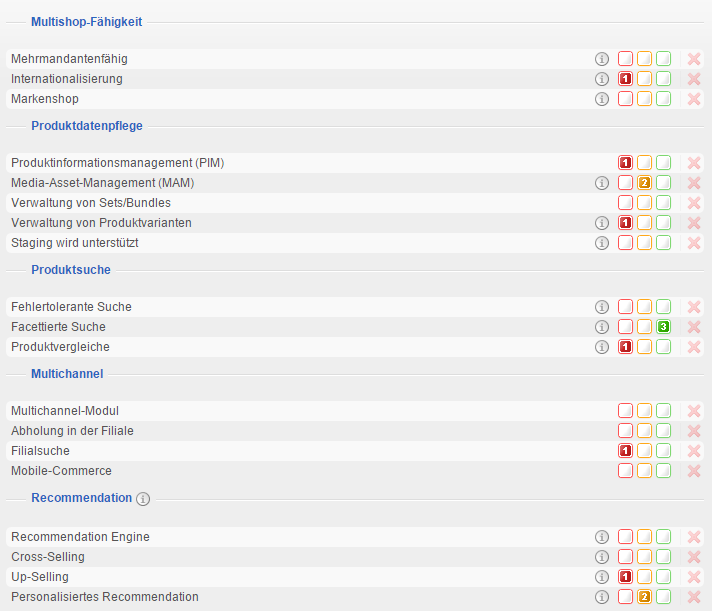
\includegraphics[width=0.7\textwidth]{images/tr14}
\end{figure}\FloatBarrier
\noindent
\begin{figure}[here!]
\centering
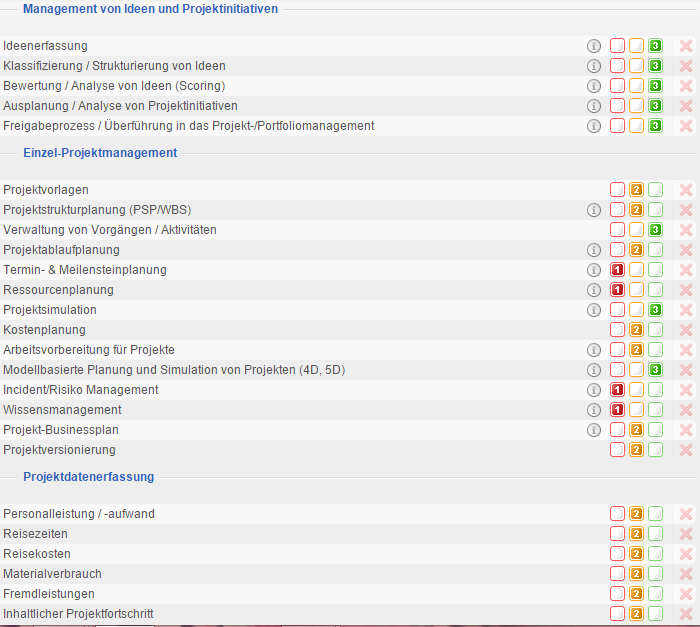
\includegraphics[width=0.7\textwidth]{images/tr15}
\end{figure}\FloatBarrier
\noindent
\begin{figure}[here!]
\centering
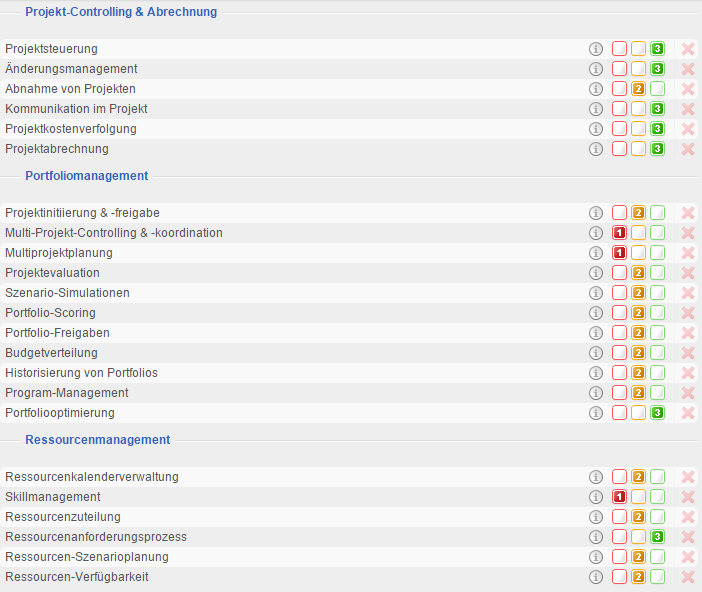
\includegraphics[width=0.7\textwidth]{images/tr16}
\end{figure}\FloatBarrier
\noindent
\begin{figure}[here!]
\centering
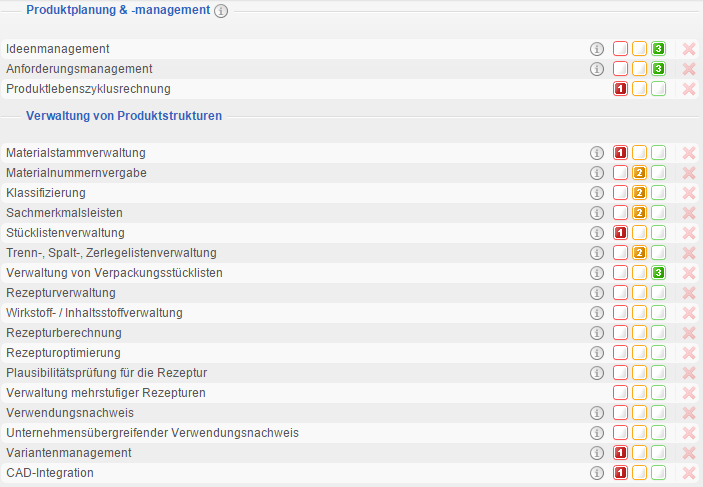
\includegraphics[width=0.7\textwidth]{images/tr17}
\end{figure}\FloatBarrier
\noindent
\begin{figure}[here!]
\centering
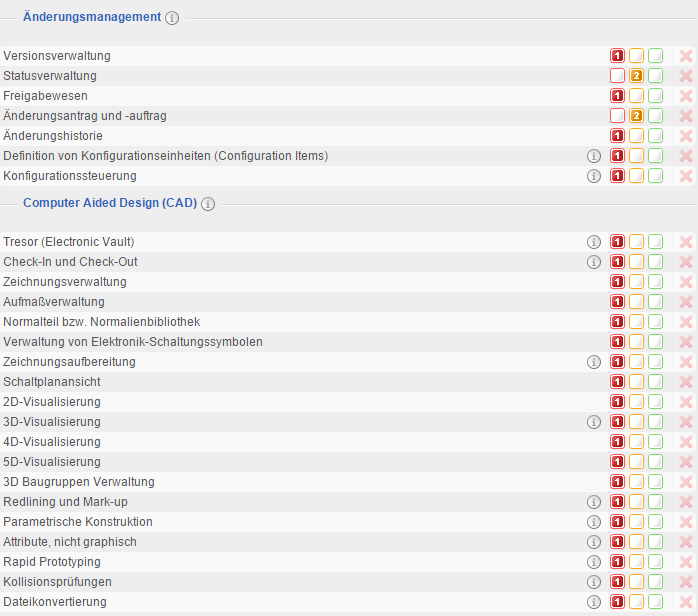
\includegraphics[width=0.7\textwidth]{images/tr18}
\end{figure}\FloatBarrier
\noindent
\begin{figure}[here!]
\centering
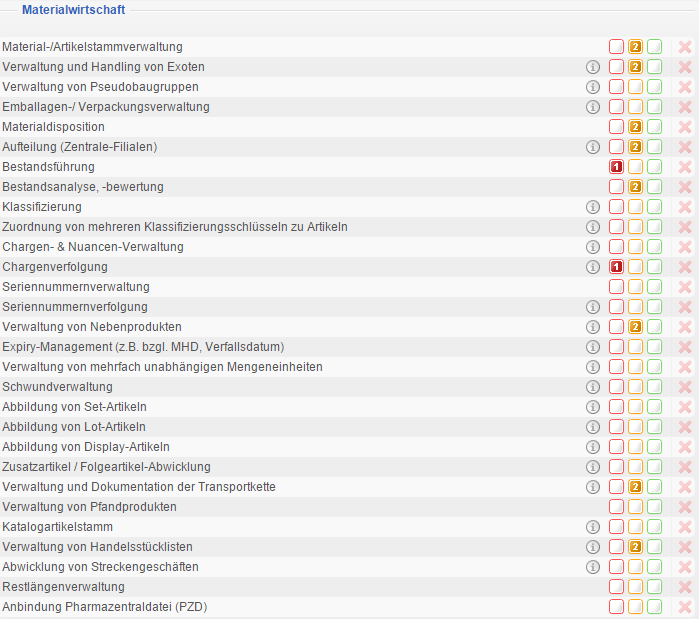
\includegraphics[width=0.7\textwidth]{images/tr19}
\end{figure}\FloatBarrier
\noindent
\begin{figure}[here!]
\centering
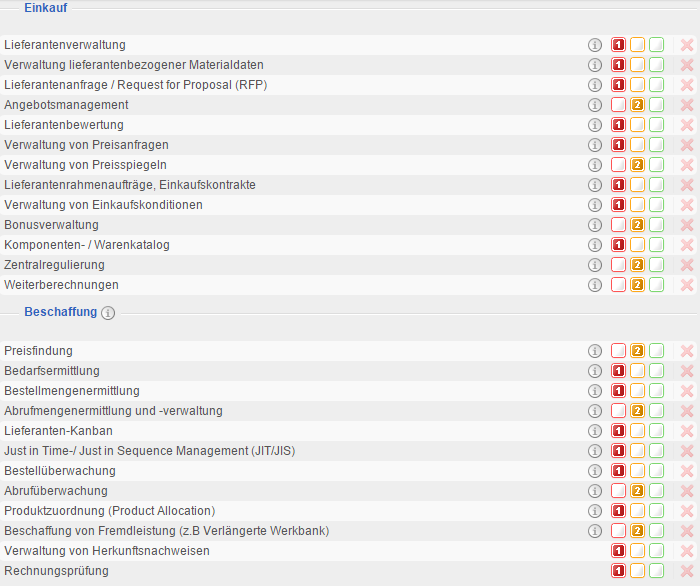
\includegraphics[width=0.7\textwidth]{images/tr20}
\end{figure}\FloatBarrier
\noindent

\begin{figure}[here!]
\centering
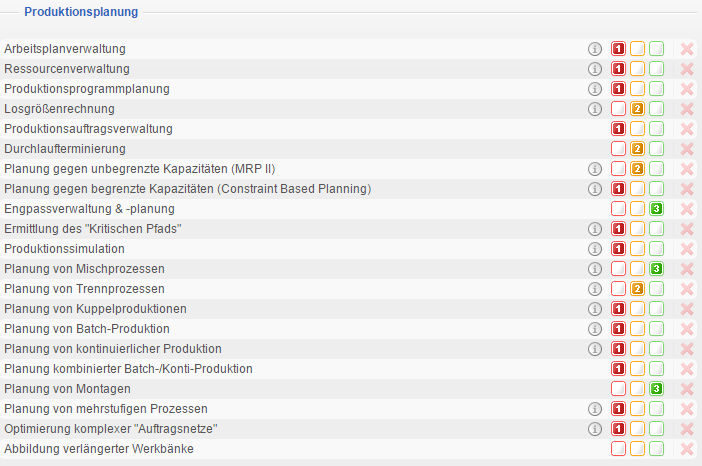
\includegraphics[width=0.7\textwidth]{images/tr21}
\end{figure}\FloatBarrier
\noindent
\begin{figure}[here!]
\centering
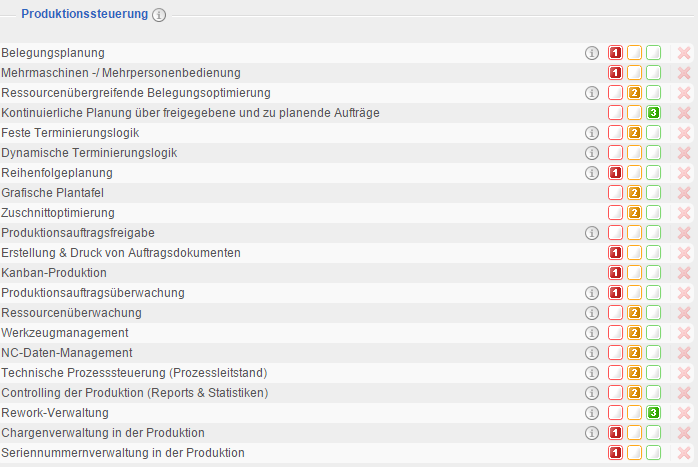
\includegraphics[width=0.7\textwidth]{images/tr22}
\end{figure}\FloatBarrier
\noindent
\begin{figure}[here!]
\centering
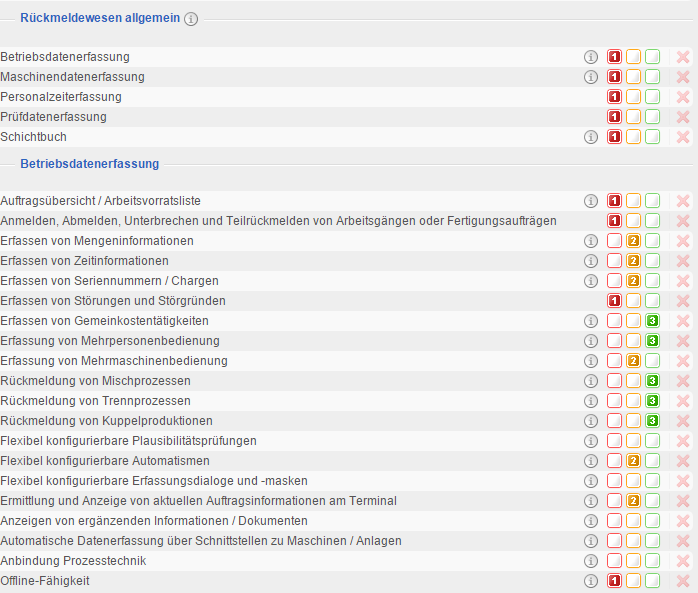
\includegraphics[width=0.7\textwidth]{images/tr23}
\end{figure}\FloatBarrier
\noindent
\begin{figure}[here!]
\centering
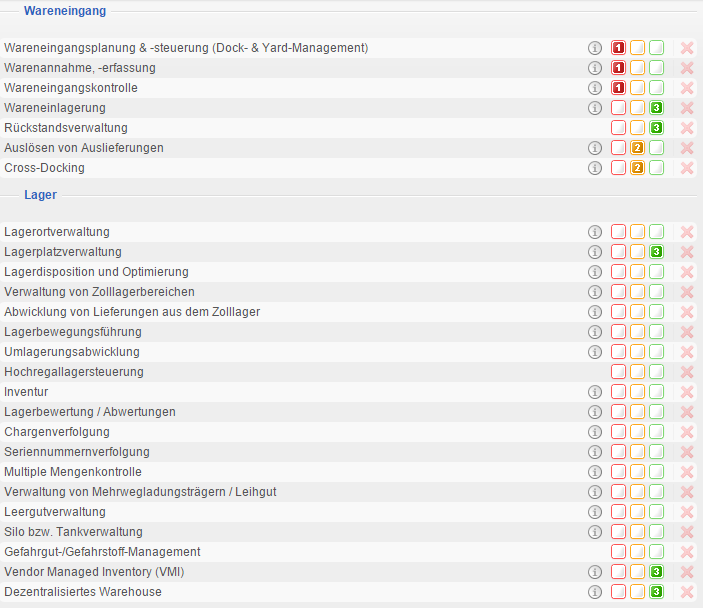
\includegraphics[width=0.7\textwidth]{images/tr24}
\end{figure}\FloatBarrier
\noindent
\begin{figure}[here!]
\centering
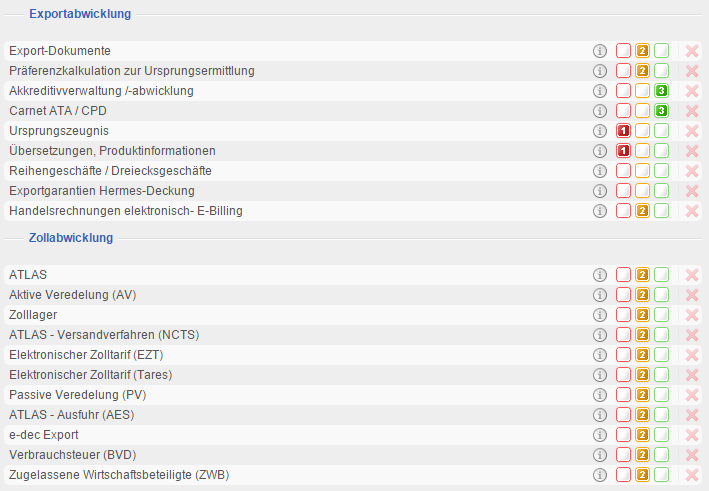
\includegraphics[width=0.7\textwidth]{images/tr25}
\end{figure}\FloatBarrier
\noindent
\begin{figure}[here!]
\centering
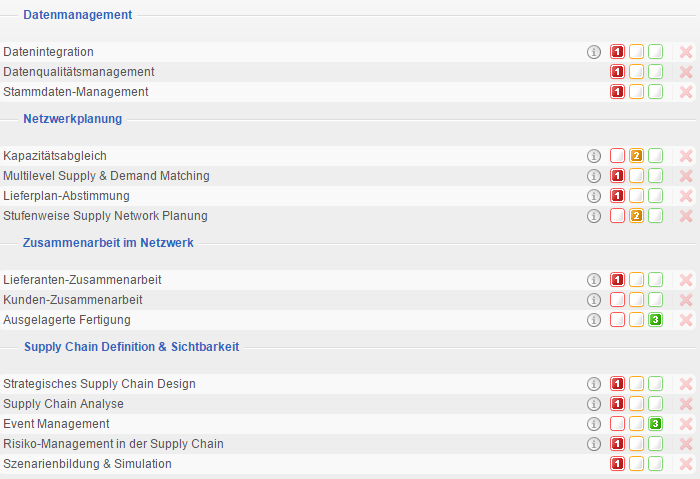
\includegraphics[width=0.7\textwidth]{images/tr26}
\end{figure}\FloatBarrier
\noindent
\begin{figure}[here!]
\centering
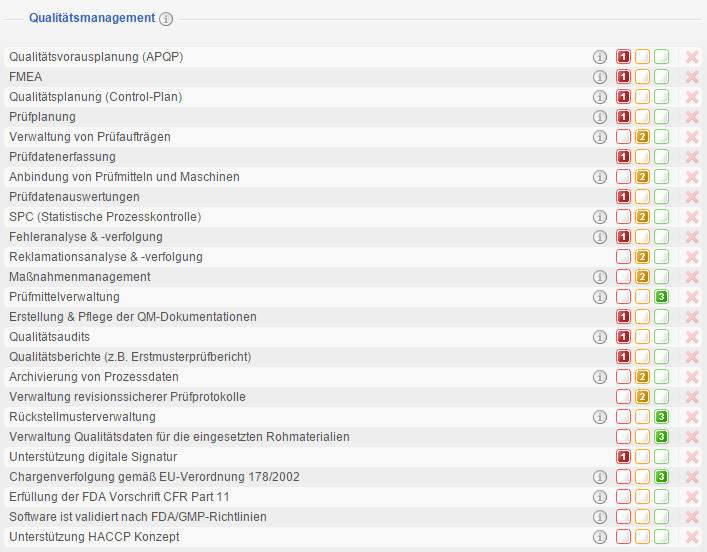
\includegraphics[width=0.7\textwidth]{images/tr27}
\end{figure}\FloatBarrier
\noindent
\begin{figure}[here!]
\centering
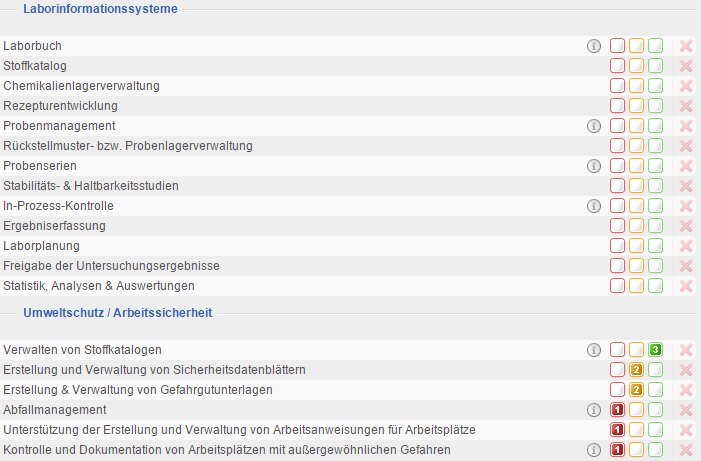
\includegraphics[width=0.7\textwidth]{images/tr28}
\end{figure}\FloatBarrier
\noindent
\begin{figure}[here!]
\centering
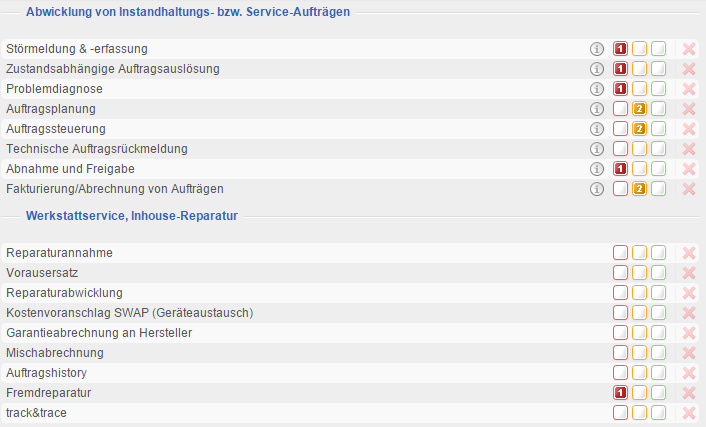
\includegraphics[width=0.7\textwidth]{images/tr29}
\end{figure}\FloatBarrier
\noindent
\begin{figure}[here!]
\centering
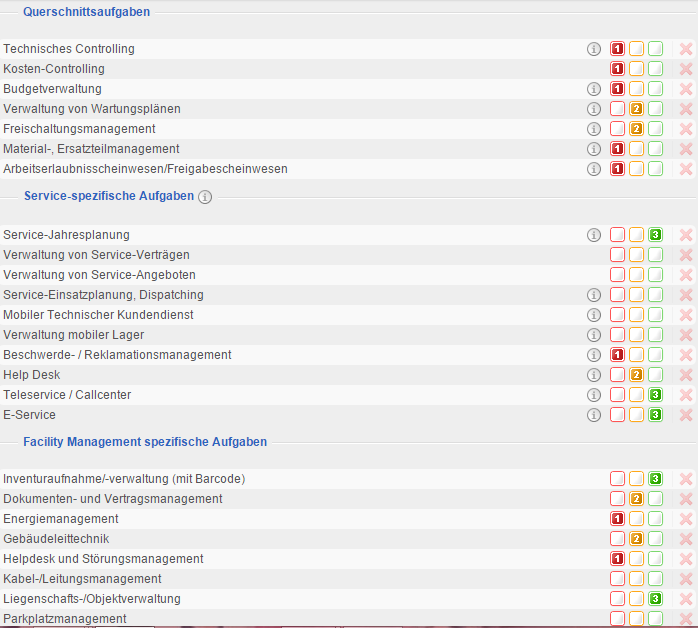
\includegraphics[width=0.7\textwidth]{images/tr30}
\end{figure}\FloatBarrier
\noindent
\begin{figure}[here!]
\centering
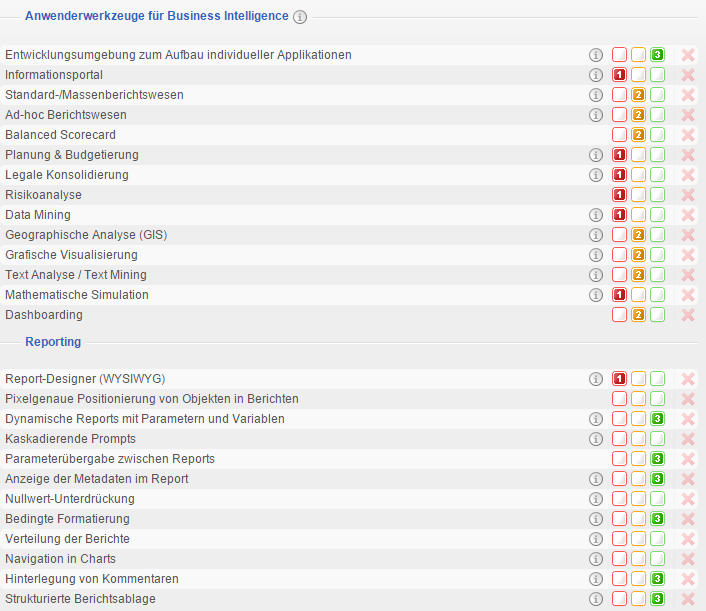
\includegraphics[width=0.7\textwidth]{images/tr31}
\end{figure}\FloatBarrier
\noindent
\begin{figure}[here!]
\centering
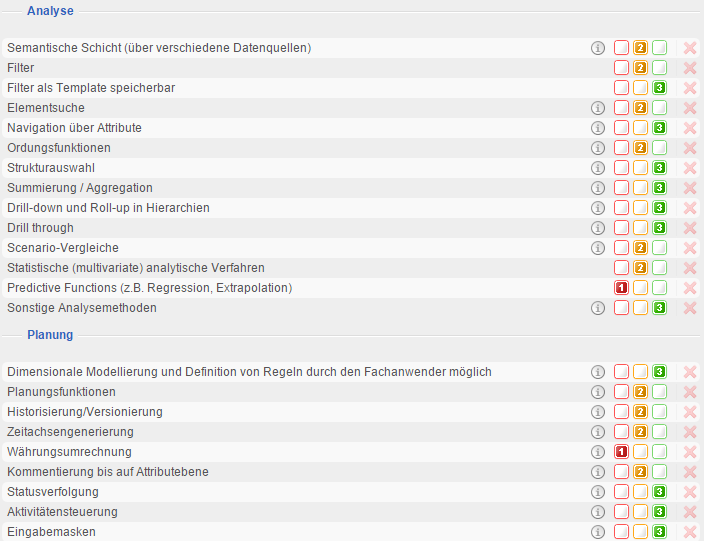
\includegraphics[width=0.7\textwidth]{images/tr32}
\end{figure}\FloatBarrier
\noindent
\begin{figure}[here!]
\centering
\includegraphics[width=0.7\textwidth]{images/tr33}
\end{figure}\FloatBarrier
\noindent
\begin{figure}[here!]
\centering
\includegraphics[width=0.7\textwidth]{images/tr34}
\end{figure}\FloatBarrier
\noindent
\begin{figure}[here!]
\centering
\includegraphics[width=0.7\textwidth]{images/tr35}
\end{figure}\FloatBarrier
\noindent
\begin{figure}[here!]
\centering
\includegraphics[width=0.7\textwidth]{images/tr36}
\end{figure}\FloatBarrier
\noindent
\begin{figure}[here!]
\centering
\includegraphics[width=0.7\textwidth]{images/tr37}
\end{figure}\FloatBarrier
\noindent
\begin{figure}[here!]
\centering
\includegraphics[width=0.7\textwidth]{images/tr38}
\end{figure}\FloatBarrier
\noindent
\begin{figure}[here!]
\centering
\includegraphics[width=0.7\textwidth]{images/tr39}
\end{figure}\FloatBarrier
\noindent
\begin{figure}[here!]
\centering
\includegraphics[width=0.7\textwidth]{images/tr40}
\end{figure}\FloatBarrier
\noindent

\begin{figure}[here!]
\centering
\includegraphics[width=0.7\textwidth]{images/tr41}
\end{figure}\FloatBarrier
\noindent
\begin{figure}[here!]
\centering
\includegraphics[width=0.7\textwidth]{images/tr42}
\end{figure}\FloatBarrier
\noindent
\begin{figure}[here!]
\centering
\includegraphics[width=0.7\textwidth]{images/tr43}
\end{figure}\FloatBarrier
\noindent
\begin{figure}[here!]
\centering
\includegraphics[width=0.7\textwidth]{images/tr44}
\end{figure}\FloatBarrier
\noindent
\begin{figure}[here!]
\centering
\includegraphics[width=0.7\textwidth]{images/tr45}
\end{figure}\FloatBarrier
\noindent
\begin{figure}[here!]
\centering
\includegraphics[width=0.7\textwidth]{images/tr46}
\end{figure}\FloatBarrier
\noindent
\begin{figure}[here!]
\centering
\includegraphics[width=0.7\textwidth]{images/tr47}
\end{figure}\FloatBarrier
\noindent
\begin{figure}[here!]
\centering
\includegraphics[width=0.7\textwidth]{images/tr48}
\end{figure}\FloatBarrier
\noindent
\begin{figure}[here!]
\centering
\includegraphics[width=0.7\textwidth]{images/tr49}
\end{figure}\FloatBarrier
\noindent
\begin{figure}[here!]
\centering
\includegraphics[width=0.7\textwidth]{images/tr50}
\end{figure}\FloatBarrier
\noindent
\begin{figure}[here!]
\centering
\includegraphics[width=0.7\textwidth]{images/tr51}
\end{figure}\FloatBarrier
\noindent
\begin{figure}[here!]
\centering
\includegraphics[width=0.7\textwidth]{images/tr52}
\end{figure}\FloatBarrier
\noindent
Die Postleitzahl der Zentrale in Wolfsburg (D) ist 38440.
\begin{figure}[here!]
\centering
\includegraphics[width=0.7\textwidth]{images/tr53}
\end{figure}\FloatBarrier
\noindent
\begin{figure}[here!]
\centering
\includegraphics[width=0.7\textwidth]{images/tr54}
\end{figure}\FloatBarrier
\noindent
\begin{figure}[here!]
\centering
\includegraphics[width=0.7\textwidth]{images/tr55}
\end{figure}\FloatBarrier
\noindent
\subsection{Auswahl}



 Microsoft Dynamics AX 2012
 
 SAP Business All-in-One

Microsoft Österreich GmbH / Dynamics NAV



\begin{figure}[here!]
\centering
\includegraphics[width=0.7\textwidth]{images/matching1}
\end{figure}\FloatBarrier
\noindent

\begin{figure}[here!]
\centering
\includegraphics[width=0.7\textwidth]{images/matching2}
\end{figure}\FloatBarrier
\noindent

\begin{figure}[here!]
\centering
\includegraphics[width=0.7\textwidth]{images/matching3}
\end{figure}\FloatBarrier
\noindent

\begin{figure}[here!]
\centering
\includegraphics[width=0.7\textwidth]{images/matching4}
\end{figure}\FloatBarrier
\noindent


\section*{Projekthandbuch}
\section*{Pflichtenheft}
\section*{Vorbereitung Kick Off Meeting}




\newpage
\listoftables
\listoffigures
\subsection{Easy Bibliography}
\begin{thebibliography}{56}

 \bibitem{ec1} 
  \textbf{Beetling back to success}, Jun 24th 2014, P.E, The Economist\\
  \textit{http://www.economist.com/blogs/schumpeter/2014/06/volkswagen-america}
  \newline last used: 07.03.2015, 13:00
  
   
 \bibitem{ec2} 
  \textbf{VW conquers the world - Germany’s biggest carmaker is leaving rivals in the dust}\\, Jul 7th 2012 , The Economist\\
  \textit{  http://www.economist.com/node/21558269}
  \newline last used: 07.03.2015, 13:07
  
    
   
 \bibitem{ec3} 
  \textbf{Europe goes electric - The Frankfurt motor show
}\\,Sep 12th 2013 , P.E., The Economist\\
  \textit{  http://www.economist.com/node/21558269}
  \newline last used: 07.03.2015, 13:09
  
   \bibitem{vsc50y} 
  \textbf{Volkswagen Share celebrates its 50th birthday}\\, Jun 4th 2011 , Volkswagen AG\\
  \textit{http://www.volkswagenag.com/content/vwcorp/info\_center/en/themes/2011/04/Volkswagen\_Share\_celebrates\_its\_50th\_birthday.html
}
  \newline last used: 07.03.2015, 13:16
  
   \bibitem{2008kurs} 
  \textbf{Volkswagen Share celebrates its 50th birthday}\\, Jun 4th 2011 , Volkswagen AG\\
  \textit{  http://www.boerse.de/boersenwissen/boersengeschichte/Kurskapriolen-der-VW-Aktie-2008-\%7C45}
  \newline last used: 07.03.2015, 13:24
  

   \bibitem{jbilanz2013vw} 
  \textbf{ABSCHLUSS VOLKSWAGEN AG }, 2013 \\
  \textit{ http://www.volkswagenag.com/content/vwcorp/info\_center/de/publications/2014/03/Financial\_Statements\_VWAG\_2013.bin.html/binarystorageitem/file/Abschluss+Volkswagen+AG+2013\_deutsch.pdf  
}
  \newline last used: 08.03.2015, 14:03
    
    
       \bibitem{aktionaersstruktur} 
  \textbf{Aktionärsstruktur Volkswagen AG}, Stand 31.12.2014 \\
  \textit{http://www.volkswagenag.com/content/vwcorp/content/de/investor\_relations/share/Shareholder\_Structure.html}
  \newline last used: 01.04.2015, 15:04
    
  \bibitem{structure1} 
  \textbf{Struktur und Geschäftstätigkeit}\\
  \textit{http://www.volkswagenag.com/content/gb2007/content/de/corporate\_governance/structure\_and\_business\_activities\_\_part\_of\_the\_management\_report\_.html}
  \newline last used: 01.04.2015, 16:47
  
  \bibitem{domavw} 
  \textbf{Aufbauorganisation der Volkswagen AG}, volkswagenag.com \\
  \textit{http://bauhaus.cs.uni-magdeburg.de:8080/miscms.nsf/FEA8C8150500AA14C1257449004F79A9/CE79949E8E27681DC12579C1006D9A27/\$FILE/Diplomarbeit\%20Oliver\%20Meier.pdf}
  \newline last used: 01.04.2015, 18:51  
  
       \bibitem{2008wtf} 
 \textbf{Short sellers make VW the world's priciest firm}, reuters.com. SARAH Marsh \\
  \textit{  http://www.reuters.com/article/2008/10/28/us-volkswagen-idUSTRE49R3I920081028}
  \newline last used: 01.04.2015, 15:39  
  
         \bibitem{aktienfotos} 
 \textbf{Vorzugs- und Stammaktien}, volkswagenag.com \\
  \textit{   http://www.volkswagenag.com/content/vwcorp/content/de/investor\_relations/share.html}
  \newline last used: 01.04.2015, 15:57
  
  \bibitem{marken} 
 \textbf{Web Ressource}, marketbusinessnews.com \\
  \textit{   http://marketbusinessnews.com/wp-content/uploads/2014/02/Volkswagen-Group-Brands.png}
  \newline last used: 01.04.2015, 16:33
  
  \bibitem{produktionsstandorte} 
 \textbf{Produktionsstandorte}, mvolkswagenag.com \\
  \textit{   http://www.volkswagenag.com/content/vwcorp/content/de/the\_group/production\_plants.html}
  \newline last used: 01.04.2015, 17:02
  
  \bibitem{struktur} 
 \textbf{Struktur und Geschäftstätigkeit}, volkswagenag.com \\
  \textit{	http://www.volkswagenag.com/content/gb2007/content/de/corporate\_governance/structure\_and\_business\_activities\_\_part\_of\_the\_management\_report\_.html}
  \newline last used: 01.04.2015, 15:57  

      \bibitem{yahoofinanzenvw} 
 \textbf{Volkswagen AG},Yahoo Finanzen \\
  \textit{  https://de.finance.yahoo.com/q/ks?s=VOW3.DE}
  \newline last used: 01.04.2015, 16:33  
  
        \bibitem{vwwebsitestrat} 
 \textbf{Volkswagen AG Strategie},volkswagenag.com \\
  \textit{http://www.volkswagenag.com/content/vwcorp/content/de/the\_group/strategy.html}
  \newline last used: 01.04.2015, 17:00  
    
      \bibitem{vwwebsitechina} 
 \textbf{Markt Spezial : China},volkswagenag.com \\
  \textit{http://www.volkswagenag.com/content/vwcorp/content/de/investor\_relations/Warum\_Volkswagen/Marke\_Focus.html
}
  \newline last used: 01.04.2015, 17:38
  \bibitem{geschdautos} 
  \textbf{Geschichte des Autos} \\
  \textit{
  	http://www.fundus.org/referat.asp?ID=11034
  }
  \newline last used: 27.03.2015, 14:23
  
  
  \bibitem{autowp} 
  \textbf{Entstehungsgeschichte von VW} \\
  \textit{
  	http://www.autowallpaper.de/Wallpaper/VW/Entstehungsgeschichte\_VW.htm
  }
  \newline last used: 27.03.2015, 14:26
  
  \bibitem{terror} 
  \textbf{Wolfgang Benz, Barbara Distel}, 2005-2009 \\
  \textit{
  	Der Ort des Terrors. Geschichte der nationalsozialistischen Konzentrationslager
  }
  
  
  \bibitem{ahwest} 
  \textbf{Volgswagen AG Geschichte} \\
  \textit{
  	http://www.autohaus-westend.de/volkswagen-ag-geschichte/
  }
  \newline last used: 27.03.2015, 13:41
  
  \bibitem{vwag} 
  \textbf{Volgswagen AG} \\
  \textit{
  	http://www.volkswagenag.com/
  }
  \newline last used: 27.03.2015, 9:13
  
  \bibitem{sud} 
  \textbf{Drastische Gewinneinbruch bei VW} \\
  \textit{
  	http://www.sueddeutsche.de/wirtschaft/geschaeftsjahr-drastischer-gewinneinbruch-bei-vw-1.814556
  }
  \newline last used: 27.03.2015, 12:11
  
  \bibitem{vwchronik} 
  \textbf{VW Chronik} \\
  \textit{
  	http://www.chronik.volkswagenag.com/
  }
  \newline last used: 29.03.2015, 12:32

\bibitem{mwpic} 
\textbf{Martin Winterkorn Bild} \\
\textit{
	http://www.blogcdn.com/de.autoblog.com/media/2011/01/martin-winterkorn-vw-volkswagen.jpg
}
\newline last used: 02.04.2015, 14:01

\bibitem{fspic} 
\textbf{Francisco Sanz Bild} \\
\textit{
	http://autogramm.volkswagen.de/07-08\_12/images/content/popups/23\_Sanz.jpg
}
\newline last used: 02.04.2015, 14:01

\bibitem{jhpic} 
\textbf{Jochem Heizmann Bild} \\
\textit{
	http://autogramm.volkswagen.de/08\_10/images/content/popups/07\_P\_heizmann.jpg
}
\newline last used: 02.04.2015, 14:02

\bibitem{ckpic} 
\textbf{Christian Klingler Bild} \\
\textit{
	http://www.produktion.de/wp-content/uploads/2014/04/christian\_klingler.jpg
}
\newline last used: 02.04.2015, 14:03

\bibitem{mmpic} 
\textbf{Matthias Mueller Bild} \\
\textit{
	http://fotos.autozeitung.de/938x704/images/bildergalerie/2015/02/porsche-matthias-mueller.jpg
}
\newline last used: 02.04.2015, 14:04

\bibitem{hnpic} 
\textbf{Horst Neumann Bild} \\
\textit{
	http://www.astroman.com.pl/img/magazyn/1376/o/Horst\_Neumann\_1.jpg
}
\newline last used: 02.04.2015, 14:04

\bibitem{arpic} 
\textbf{Andreas Renschler Bild} \\
\textit{
	http://transportnet.se/files/2014/02/AndreasRenschler.jpg
}
\newline last used: 02.04.2015, 14:04

\bibitem{hppic} 
\textbf{Hans Poetsch Bild} \\
\textit{
	http://www.automobil-produktion.de/uploads/2011/03/vw\_poetsch-229x300.jpg
}
\newline last used: 02.04.2015, 14:05

\bibitem{rspic} 
\textbf{Rupert Stadler Bild} \\
\textit{
	http://www.matthiashaslauer.com/corporate/stadler/haslauer\_1.jpg
}
\newline last used: 02.04.2015, 14:05


\end{thebibliography}
\end{document}
%img : httpmarkets.ft.comresearchMarketsTearsheetsSummarys=VOWBER vwdax.PNG
% http://www.statista.com/statistics/257660/passenger-car-sales-in-selected-countries/ salesla
% http://www.statista.com/statistics/232958/revenue-of-the-leading-car-manufacturers-worldwide/ revenu
